\documentclass[12pt, a4paper]{report}

\usepackage[utf8]{inputenc}
\usepackage[french, arabic, main=english]{babel}
\usepackage{csquotes}
\usepackage[LAE, T1]{fontenc}
\usepackage{array}
\usepackage{amsmath, amssymb, amsfonts, amsthm}
\usepackage{bbm}
\usepackage[dvipsnames,svgnames]{xcolor}
\usepackage{fancyhdr}
\usepackage{graphicx}
\graphicspath{{assets/images}{assets/pdf}{assets/python}}
\usepackage[inline]{enumitem}
\usepackage{import}
\usepackage{colonequals}
\usepackage{hyperref}
\hypersetup{%
    colorlinks=true,
    linkcolor=black,
    urlcolor=black,
    citecolor=DarkGreen,
    pdfauthor={Mohammed Belgoumri},
    pdfkeywords={this is a kw}
}
\usepackage{cleveref}
\usepackage[top=2.5cm,bottom=2.5cm,right=2.5cm,left=2.5cm]{geometry}
\usepackage{appendix}
\usepackage{wrapfig}
\usepackage{cprotect}
\import{preambule}{tikz}

\newlength\figureheight
\newlength\figurewidth

% \usepackage[backend=biber, style=apa]{biblatex}

\usepackage[backend=biber,style=numeric]{biblatex}
\addbibresource{references.bib}

\usepackage{etoolbox}

\usepackage{caption}

\import{preambule}{codestyle}
%% Algorithm style
\usepackage[ruled,linesnumbered,nosemicolon]{algorithm2e}
\SetFuncArgSty{}
\definecolor{codegreen}{rgb}{0,0.6,0}
\newcommand{\mycomntsty}[1]{\texttt{\textcolor{codegreen}{#1}}}
\newlength{\commentWidth}
\setlength{\commentWidth}{7cm}
\SetCommentSty{mycomntsty}
\newcommand{\atcp}[1]{\tcp*[r]{\makebox[\commentWidth]{#1\hfill}}}
% no line break version of \atcp
\newcommand{\atcpl}[1]{\tcp*[f]{\makebox[\commentWidth]{#1\hfill}}}

\usepackage{arabtex}
\usepackage{utf8}
\setcode{utf8}

\usepackage{afterpage}
\usepackage{float}
\usepackage{subcaption}



\usepackage{stmaryrd}
\usepackage{bookmark}
\usepackage{booktabs}
\usepackage{stackengine}
\usepackage{adjustbox}
\usepackage{footnote}


\usepackage{geometry}
\usepackage{multirow}
\usepackage{array}
\usepackage{booktabs} % For better horizontal lines
\usepackage{makecell}



% pakages for header writing 

\usepackage{fancyhdr}
\pagestyle{fancy}
\fancyhf{}

% Header: current chapter title (automatically set by \chapter)
\fancyhead[L]{\nouppercase{\leftmark}}
\fancyfoot[C]{\thepage}

\renewcommand{\headrulewidth}{0.4pt}

% Make sure plain pages (e.g. at start of chapters) use same style
\fancypagestyle{plain}{
  \fancyhf{}
  \fancyhead[L]{\nouppercase{\leftmark}}
  \fancyfoot[C]{\thepage}
  \renewcommand{\headrulewidth}{0.4pt}
}



\usepackage{enumitem}



\usepackage{mathptmx} % or use \usepackage{times}





\makesavenoteenv{tabular}
\makesavenoteenv{table}


\setlength{\parskip}{.4cm}
\import{preambule}{theorems}

% Fix the problem of \times (caused by babel or arabtex)
\renewcommand{\times}{\mathbin{\mathsf{x}}}


% Number sets
\newcommand{\complexes}{\mathbb{C}}
\newcommand{\reals}{\mathbb{R}}
\newcommand{\rationals}{\mathbb{Q}}
\newcommand{\integers}{\mathbb{Z}}
\newcommand{\naturals}{\mathbb{N}}
\newcommand{\field}{\mathbb{K}}


% Problems/ complexity classes
\newcommand{\TSP}{\textsf{TSP}}
\newcommand{\classP}{\textsf{P}}
\newcommand{\classNP}{\textsf{NP}}
\newcommand{\classNPO}{\textsf{NPO}}

% Math operators
\newcommand{\argmin}{\operatornamewithlimits{argmin}}
\newcommand{\argmax}{\operatornamewithlimits{argmax}}
\newcommand{\diff}[1]{\mathrm{d}#1}
\newcommand{\pdiff}[1]{\partial#1}


% default greeks
\let\uglyepsioln\epsilon
\let\epsilon\varepsilon

\let\roundphi\phi
\let\phi\varphi

% Landau notation
\newcommand{\bigO}[1]{\mathcal{O}\left(#1\right)}

% Probability
\newcommand{\prob}{\operatornamewithlimits{\mathbb{P}}}
\newcommand{\esp}{\operatornamewithlimits{\mathbb{E}}}

% Linear algebra
\newcommand{\tr}{\operatorname{tr}}


% ML
\newcommand{\softmax}{\operatorname{softmax}}
\newcommand{\relu}{\operatorname{ReLU}}

%citation style
\let\barecite\cite
\let\cite\parencite

\import{preambule}{abbreviations}



% !TEX root = main.tex
\begin{document}
\setcounter{tocdepth}{2}
\afterpage{
  \newgeometry{top=0.6in,bottom=0.6in,right=1in,left=1in}
  \begin{titlepage}
    \pagenumbering{gobble}
    % \phantomsection\addcontentsline{toc}{chapter}{Cover page}

    \centering
    {\small République Algérienne Démocratique et Populaire}\\
    \RL{الجمهورية الجزائرية الديـموقراطية الشعبية}\\
    {\small Ministère de l'Enseignement Supérieur et de la Recherche Scientifique}\\
    \RL{وزارة التعليم العالي والبحث العلمي}\\
    \rule{\linewidth}{0.3mm} \\[0.4cm]

    \begin{minipage}{5cm}
      \begin{flushleft}
        
\includegraphics[width=4.9cm]{assets/images/esi_logo.png}
      \end{flushleft}
    \end{minipage}\hfill
    %%
    \begin{minipage}{10cm}
      \begin{flushright}
        \RL{المدرسة الوطنية للإعلام الآلي}\\
        (\RL{المعهد الوطني للتكوين في الإعلام الآلي سابقا})\\
        {\small École nationale Supérieure d'Informatique}\\[0.1cm]
        {\small ex. INI (Institut National de formation en Informatique)}\\[0.1cm]
      \end{flushright}
    \end{minipage}\hfill\\
    %%
    \vspace{20mm}
    %%
   {\large \bfseries Master’s Report}\\[0.5cm]
{\large \bfseries In order to obtain a Master’s degree in Computer Science }\\[0.5cm]
{\large \bfseries Major: Computer Systems and Software (SIL)\\ }


    \vspace{10mm}

    % Title
    \rule{\linewidth}{0.3mm} \\[0.4cm]
    {
    \Large \bfseries
    Drone and Satellite-Based Remote Sensing for Early Wheat Disease Detection: A Literature Review.\\
    }
    %%
    \rule{\linewidth}{0.3mm} \\[1cm]

    \vspace{10mm}

    % Author and supervisor
    \noindent
    \begin{minipage}{0.6\textwidth}
      \vspace{-7mm}
      \begin{flushleft} \large
        \emph{Written By:}\\
        \textsc{Abbaci} Zoulikha \\
        \href{mailto:kz_abbaci@esi.dz}{\verb!kz\_abbaci@esi.dz!} \\[0.3cm]
        \textsc{Bellali} Amira \\
        \href{mailto:ka_bellali@esi.dz}{\verb!ka\_bellali@esi.dz!}
      \end{flushleft}
    \end{minipage}
    %%
    \begin{minipage}{0.35\textwidth}
      \begin{flushright} \large
        \begin{flushleft} \large
          \emph{Supervised By:} \\
          Dr. \textsc{Bessah} Naima\\
          \href{mailto:n_bessah@esi.dz}{\verb!n\_bessah@esi.dz!}\\[0.3cm]
          Dr. \textsc{Sehad} Abdenour\\
          \href{mailto:a_sehad@esi.dz}{\verb!a\_sehad@esi.dz!}
        \end{flushleft}
      \end{flushright}
    \end{minipage}\\[1cm]

    % \begin{minipage}{.7\linewidth}
    %   \begin{center}
    %     \begin{flushleft}
    %       \emph{Soutenu le 22 juin 2025, devant le jury composé de:}\\
    %       Dr. \textsc{Chebieb} AbdelKrim (ESI): Président\\
    %       Dr. \textsc{Hamani} Nacer (ESI): Rapporteur\\
    %       Dr. \textsc{Charabi} Leila (ESI): Examinateur\\
    %     \end{flushleft}
    %   \end{center}
    % \end{minipage}

    \vfill

    {\large Cohort: 2023/2024}
  \end{titlepage}
  \restoregeometry
}

\renewcommand{\headrulewidth}{0pt}
\fancypagestyle{plain}{\fancyhf{}\cfoot{\thepage}}
% \ \vfill{}
\begin{center}
    {
        \Large\bfseries
        \RL{إهـداء}
    }
\end{center}

\begin{RLtext}
    إلـى أبـي وأمـي، صـاحـبـي الـفـضـل عـلـي بـعـد الـلـه،
    
    إلـى أخـي وأخـتـيّ وجـمـيـع أهـلـي،

    إلـى شـوقـي، أعـز أصـدقـائـي،
    
    إلـى أولـئـك الـذيـن سـألـت عـونـهـم كـلـمـا أشـكـل عـلـيّ أمـر
    
    وشـاركـونـي فـرحـة كـل نـجـاح،
    
    إلـيـكـم جـمـيـعـا، أهـدي هـذا الـعـمـل.
    أنـتـم مـن شـاركـتـمـونـي تـعـبـه وسـهـره وهـمـه،
    ولـيـس مـن أحـد أحـق مـنـكـم أن يـشـاركـنـي فـرحـتـه.
\end{RLtext}

% \vfill{}
\pagebreak
\begin{center}
    {%
        \Large\bfseries
        Acknowledgments
    }
\end{center}

\noindent
% You can add your paragraph(s) here, for example:
In the name of Allah, the Most Gracious, the Most Merciful, we begin by expressing our sincere gratitude to all those who have supported us throughout the completion of this master’s report.

Above all, we are thankful to Allah for granting us the patience, strength, and clarity to persevere through each challenge. His guidance has been our greatest source of hope and resilience.

Our heartfelt thanks go to Madam Bessah Naima and Mr. Sahed Abdenour, whose mentorship, insightful advice, and continuous encouragement have been instrumental in shaping the quality of our work. Their dedication and expertise have left a lasting impact on our academic and personal growth.

We are deeply indebted to our mothers, whose unwavering love, sacrifices, and prayers have sustained us through every step of this journey. Their support has been a pillar of strength.

To our fathers, we express our sincere appreciation for their constant belief in us, their wise counsel, and their motivation, which have inspired us to aim higher and stay determined.

Finally, we extend our gratitude to all who contributed, in ways big or small, to the realization of this work. May Allah bless you all abundantly, reward your kindness, and continue to guide you on the path of goodness.
Ameen.
% \ \vfill{}
\begin{abstract}
    \thispagestyle{plain}
    \pagenumbering{roman}
    \setcounter{page}{2}
    \phantomsection\addcontentsline{toc}{chapter}{\abstractname}

    Wheat is a vital crop that significantly contributes to global food security, yet its production is increasingly threatened by various diseases. Traditional detection and management approaches often fall short due to their reliance on manual inspection and delayed intervention. In response, the integration of smart agricultural technologies, particularly remote sensing and artificial intelligence has emerged as a powerful solution for early and accurate disease detection. This report explores the application of remote sensing data in combination with machine learning and deep learning techniques to address the challenges of wheat disease monitoring. It presents a comprehensive overview of imaging technologies such as RGB, thermal, multispectral, and hyperspectral cameras, as well as data collection platforms including satellites, aircraft, and UAVs. The study examines the full workflow from image acquisition and preprocessing to feature extraction and model-based classification using a variety of machine learning and deep learning models. It also explains how combining data from different sources can improve detection accuracy, and highlights future opportunities to use these technologies for more efficient and sustainable farming.    
    %%
    \\ [2cm]
    %%
    \rule{\linewidth}{1pt}

    \textbf{Keywords --- } Wheat disease early detection, Unmanned Aerial Vehicles (UAVs), Satellite, Remote sensing, Precision agriculture, Machine learning (ML), Deep learning (DL), Hyperspectral imaging, Vegetation indices (NDVI, NDRE).\\
    \rule{\linewidth}{1pt}
\end{abstract}


\begin{otherlanguage}{french}
    \begin{abstract}
        \thispagestyle{plain}
        \pagenumbering{roman}
        \setcounter{page}{1}
        \phantomsection\addcontentsline{toc}{chapter}{\abstractname}

        Le blé est une culture essentielle qui contribue de manière significative à la sécurité alimentaire mondiale, mais sa production est de plus en plus menacée par diverses maladies. Les méthodes traditionnelles de détection et de gestion, reposant souvent sur des inspections manuelles et des interventions tardives, montrent leurs limites. Face à ces défis, l’intégration des technologies agricoles intelligentes, notamment la télédétection et l’intelligence artificielle, s’impose comme une solution efficace pour une détection précoce et précise des maladies. Ce rapport explore l’utilisation des données de télédétection combinées à des techniques d’apprentissage automatique et d’apprentissage profond pour surveiller les maladies du blé. Il propose un aperçu complet des technologies d’imagerie telles que les caméras RGB, thermiques, multispectrales et hyperspectrales, ainsi que des plateformes de collecte de données, incluant les satellites, les avions et les drones (UAVs). L’étude examine l’ensemble du processus, de l’acquisition et du prétraitement des images à l’extraction des caractéristiques et à la classification basée sur différents modèles d’apprentissage. Elle met également en évidence comment la combinaison de données provenant de différentes sources peut améliorer la précision de la détection, tout en soulignant les perspectives futures pour une agriculture plus efficace et durable.
        %%
        \ \\[2cm]
        %%
        \rule{\linewidth}{1pt}

        \textbf{Mots clés --- } Détection précoce des maladies du blé, Véhicules aériens sans pilote (UAV), Satellite, Télédétection, Agriculture de précision, Apprentissage automatique (ML), Apprentissage profond (DL), Imagerie hyperspectrale, Indices de végétation (NDVI, NDRE).\\
        \rule{\linewidth}{1pt}
    \end{abstract}

\end{otherlanguage}
\renewcommand{\abstractname}{\RL{مـلـخـص}}
\afterpage{
    \newgeometry{top=-2cm}
    \begin{abstract}
        \thispagestyle{plain}
        \pagenumbering{roman}
        \setcounter{page}{3}
        \phantomsection\addcontentsline{toc}{chapter}{\textRL{مـلـخـص}}
        \begin{RLtext}
            القمح هو محصول حيوي يسهم بشكل كبير في الأمن الغذائي العالمي، ومع ذلك فإن إنتاجه مهدد بشكل متزايد من قبل العديد من الأمراض. غالبًا ما تكون أساليب الكشف والإدارة التقليدية غير كافية نظرًا لاعتمادها على الفحص اليدوي والتدخل المتأخر. استجابةً لذلك، ظهرت تقنيات الزراعة الذكية، وخاصة الاستشعار عن بُعد والذكاء الاصطناعي، كحل قوي للكشف المبكر والدقيق عن الأمراض. يستعرض هذا التقرير تطبيق بيانات الاستشعار عن بُعد بالاشتراك مع تقنيات التعلم الآلي والتعلم العميق للتصدي لتحديات مراقبة أمراض القمح. يقدم التقرير لمحة شاملة عن تقنيات التصوير مثل كاميرات RGB، والتصوير الحراري، والمجموعة الطيفية المتعددة، والكاميرات الطيفية الفائقة، بالإضافة إلى منصات جمع البيانات مثل الأقمار الصناعية والطائرات والطائرات بدون طيار (UAVs). كما يفحص الدراسة سير العمل الكامل من الحصول على الصور والمعالجة الأولية لها، إلى استخراج الميزات وتصنيف البيانات باستخدام مجموعة من نماذج التعلم الآلي والتعلم العميق. كما يشرح كيف يمكن لتحليل البيانات من مصادر متعددة تحسين دقة الكشف، ويبرز الفرص المستقبلية لاستخدام هذه التقنيات من أجل الزراعة الأكثر كفاءة واستدامة.        \end{RLtext}
        \hspace*{0mm}\rule{\linewidth}{1pt}
        \begin{RLtext}
            \textbf{الـكـلـمـات الـمـفـتـاحـيـة ـــ }الكشف المبكر عن أمراض القمح، الطائرات بدون طيار ، الأقمار الصناعية، الاستشعار عن بعد، الزراعة الدقيقة، التعلم الآلي ، التعلم العميق ، التصوير الطيفي الفائق، مؤشرات الغطاء النباتي .\\
        \end{RLtext}
        \rule{\linewidth}{1pt}
    \end{abstract}
    \restoregeometry
}
% \vfill{}
\afterpage{
    \newgeometry{bottom=3cm}
    \tableofcontents
    \addcontentsline{toc}{chapter}{Contents}
    \listoffigures
    \addcontentsline{toc}{chapter}{List of figures}
    \lstlistoflistings
    \addcontentsline{toc}{chapter}{List of Table}
    \listofalgorithms
    \addcontentsline{toc}{chapter}{List of Algorithms}
}
% \printabbreviations
\cleardoublepage
\printabbreviations[
    title=Abbreviations,
    toctitle=Abbreviations,
    style=long,nonumberlist
]
\restoregeometry
\pagenumbering{arabic}
\chapter*{General introduction}
\addcontentsline{toc}{chapter}{General introduction}
\label{chap.intro}

Wheat is a staple food crop, crucial to global food security. However, wheat production is persistently threatened by a range of diseases and pests that can significantly reduce yield and quality. Traditionally, farmers have relied on manual inspection and chemical treatments to manage crop diseases, but these methods are often time-consuming, imprecise, and unsustainable in the long term.

In recent years, the rise of smart agriculture has introduced innovative approaches to crop monitoring and disease management. In particular, the integration of remote sensing technologies with machine learning (ML) and deep learning (DL) algorithms has enabled a paradigm shift in how agricultural data is collected, processed, and utilized.

Remote sensing platforms—including satellites, drones (UAVs), and ground-based sensors—allow the non-invasive acquisition of multispectral, hyperspectral, and thermal imagery, which can reveal subtle signs of plant stress and disease that are invisible to the naked eye. When combined with ML and DL models, this data can be automatically analyzed to classify disease types, detect early infections, and support real-time decision-making at scale.

This report investigates the synergy between remote sensing and artificial intelligence in the context of wheat disease detection. It provides:

An overview of common wheat diseases and their agricultural impact.

\begin{itemize}
    \item A detailed examination of Deep Learning methods and their application in computer vision tasks such as image classification, object detection, and segmentation.
    \item A technical survey of remote sensing tools and platforms used for agricultural monitoring.
    \item A discussion on workflows for integrating imagery with AI models, feature extraction methods, and data fusion strategies.
  \end{itemize}
  
By exploring these technologies and their integration, this work highlights the potential of intelligent systems to improve disease management, reduce crop losses, and contribute to more resilient and sustainable agriculture.
% === Première Partie: État de l'art ===
\part{State of Art}

\chapter{Applications of Deep Learning in Visual Recognition of Wheat Diseases}

\section{Introduction}
The spread of wheat diseases poses serious threats to agricultural productivity and food security. Early and accurate detection is essential for timely intervention and disease management. In this context, deep learning has emerged as a powerful approach to support smart agriculture by enabling automated, data-driven solutions.

This chapter focuses on the application of deep learning techniques to visual data, particularly images captured in the field. It highlights three key computer vision tasks used in precision agriculture: image classification, image segmentation, and object detection. These tasks allow machines to recognize disease types, locate affected areas on plant surfaces, and detect objects such as crops or weeds in complex environments. The chapter begins with the fundamentals of deep neural networks and proceeds to how they are used for agricultural image analysis. It also introduces practical techniques like transfer learning and fine-tuning, which help adapt models to specific agricultural datasets.

\section{Distinctions Between Deep Learning and Machine Learning}
Deep learning is a subset of machine learning that uses deep neural networks to automatically learn complex patterns from large, unstructured data like images, text, and audio. Unlike traditional machine learning, which requires manual feature extraction and works best with smaller, structured datasets, deep learning eliminates this need and can handle large datasets with significant computational power, often using GPUs. While machine learning is suitable for tasks like predictive analytics, deep learning excels in applications such as image recognition, speech processing, and natural language understanding \parencite{AlvarezVanhard2021}.


\section{Deep Learning Fundamentals}
In this section, we introduce the core principles of deep learning, focusing on deep neural networks (DNNs) and their role in learning complex patterns from data. We explore the structure and components of neural networks, the learning process, optimization techniques, and model evaluation methods. Additionally, we highlight regularization strategies to prevent overfitting.

\subsection{Deep Neural Network Basics (DNN)}
Neural networks form the backbone of deep learning, enabling machines to learn patterns and make predictions from data. Inspired by the structure of the human brain, these networks consist of interconnected layers of artificial neurons that hierarchically process information.

\subsubsection{Definition of DNN}

Before defining deep neural networks, we first need to understand two essential components: 
\begin{itemize}
    \item \textbf{Artificial neuron}: An artificial neuron is the basic building block of artificial neural networks, designed based on the structure and functionality of biological neurons. It receives weighted inputs, processes them through a transfer function, and outputs the result. The artificial neuron model simplifies the biological process where information is received through dendrites, processed in the soma, and transmitted via the axon, as shown in Figure~\ref{fig:figure01} \parencite{krenker2011introduction}.
    
    \item \textbf{Layer}: A layer in a neural network is a set of neurons that perform a specific operation on the data \parencite{bengio2017deep}.
\end{itemize}

\begin{figure}[H] % 'H' needs \usepackage{float}
    \centering
    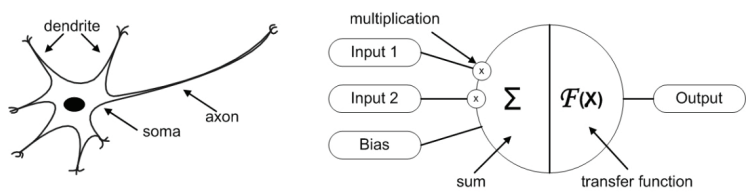
\includegraphics[width=0.6\textwidth]{chapters/chapter1/images/Figure01.png}
    \caption{Biological Neuron Structure and Its Mathematical Model Representation \parencite{krenker2011introduction}.}
    \label{fig:figure01}
\end{figure}


By combining multiple layers of interconnected artificial neurons, we arrive at the concept of a Deep Neural Network (DNN). A DNN is a neural network that contains multiple hidden layers between the input and output layers. These additional layers enable the network to learn complex patterns and high-level features from data. Each layer transforms its input into a more abstract representation, improving the network’s ability to recognize intricate structures and relationships \parencite{li2021water}.
\subsubsection{Structure of DNN}
A neural network consists of three main layers \parencite{ren2023review}:

\noindent
\textbf{The input layer:} Represents the features of the input data, such as pixel values in an image, denoted as a vector 
\[
X = [x_1, x_2, \dots, x_n].
\]

\noindent
\textbf{The hidden layers:} Process this input using weighted connections and biases, computed as:
\[
z = W \cdot X + b_z \tag{1}
\]
\[
F(z) = a \tag{2}
\]
where:
\begin{itemize}
    \item $W$ is the weight matrix,
    \item $b$ is the bias vector,
    \item $z$ is the pre-activation value,
    \item $F(z)$ is the activation function applied to $z$.
\end{itemize}

Each neuron in the hidden layers applies an activation function to capture complex patterns.

\noindent
\textbf{The output layer:} Generates the network's prediction, with the number of neurons corresponding to the specific task, such as one neuron for binary classification or multiple neurons for multiclass classification.



% \begin{figure}[H] % 'H' needs \usepackage{float}
%     \centering
%     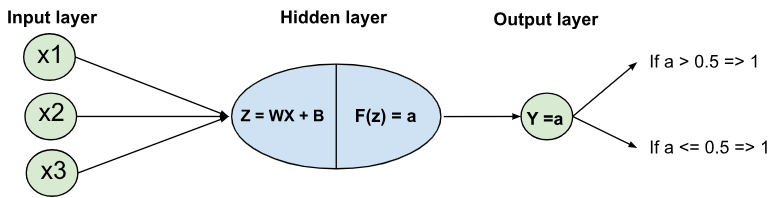
\includegraphics[width=0.6\textwidth]{chapters/chapter1/images/Figure02.png}
%     \caption{The structure of a Neural Network in the binary classification task.}
%     \label{fig:figure02}
% \end{figure}

\subsubsection{Activation Functions}
An activation function (AF) is a mathematical function applied to a neuron's output in a neural network to introduce non-linearity. Without an activation function, a neural network with multiple layers would behave like a single-layer perceptron, limiting its ability to model complex relationships \parencite{dubey2022activation}. Activation functions decide whether a neuron should be activated based on its input. 

Table \ref{tab:activation-functions} summarizes the most commonly used activation functions, their formulas, ranges, and typical use cases in deep neural networks.



\begin{table}[htbp]
    \caption{Common Activation Functions in Deep Learning \parencite{dubey2022activation}}
    \centering
    \resizebox{\textwidth}{!}{%
    \begin{tabular}{|p{3cm}|p{4.5cm}|p{3cm}|p{3.5cm}|}
    \hline
    \textbf{Activation Function} & \textbf{Formula} & \textbf{Range} & \textbf{Usage} \\
    \hline
    Sigmoid                      & $\text{Sigmoid}(x) = \frac{1}{1+e^{-x}}$         & [0, 1]               & Commonly used in binary classification problems, especially in the output layer of models predicting probabilities. \\
    \hline
    Tanh (Hyperbolic Tangent)     & $\tanh(x) = \frac{e^{x} - e^{-x}}{e^{x} + e^{-x}}$ & [-1, 1] & Often used in hidden layers of neural networks, as it outputs values centered around zero, which helps in reducing bias during optimization. \\
    \hline
    ReLU (Rectified Linear Unit)  & $\relu(x) =\text{max}(0, x)$            & [0, $\infty$)        & Widely used in hidden layers of deep neural networks due to its simplicity and effectiveness in handling the vanishing gradient problem. \\
    \hline
    Softmax & $\text{Softmax}(x_i) = \frac{e^{x_i}}{\sum_j e^{x_j}}$, where $x_i$: current element, $x_j$: all elements in the vector. & (0, 1) (outputs sum to 1) & Used in the output layer for multi-class classification. \\
    \hline

    \end{tabular}%
    }
    \label{tab:activation-functions}
\end{table}


    
\subsection{Learning Process in Deep Neural Networks}

In the information processing flow within an artificial neuron, several elements, known as parameters, are learned from the training data. These parameters include \parencite{Kelleher2019}:
\begin{itemize}
    \item \textbf{Weights}: Weights control the amount of each input feature that passes through the neuron. They represent the coefficients of the connections between neurons in the layers of a neural network. Weights are essential for determining the influence of each input on the output.
    
    \item \textbf{Biases}: Biases are values added to the outputs of the neurons before applying the activation function. They allow the network to shift the activation function, providing more flexibility to the model.
\end{itemize}

The learning process in neural networks involves training the model to map input data to desired outputs. This is achieved through the mechanisms of forward propagation and backward propagation, along with optimization techniques that refine the network's parameters (weights and biases) to minimize the error \parencite{Kelleher2019}:
\begin{itemize}
    \item \textbf{Forward Propagation}: In forward propagation, the input data passes through the network layer by layer. Each neuron in a layer performs a weighted sum of its inputs, applies an activation function, and passes the result to the next layer. The process continues until the output layer is reached and a prediction is made.
    
    \item \textbf{Backward Propagation}: Backward propagation (or backpropagation) is used to update the network's weights. After calculating the error (the difference between the predicted and actual output), the error is propagated back through the network. The weights are adjusted based on the gradient of the error with respect to each weight, using optimization algorithms like gradient descent.
\end{itemize}

Figure \ref{fig:figure03} below provides a visual representation of the learning process in a neural network, illustrating the flow of information from the input layer through multiple hidden layers to the output layer.


\begin{figure}[H] % 'H' needs \usepackage{float}
    \centering
    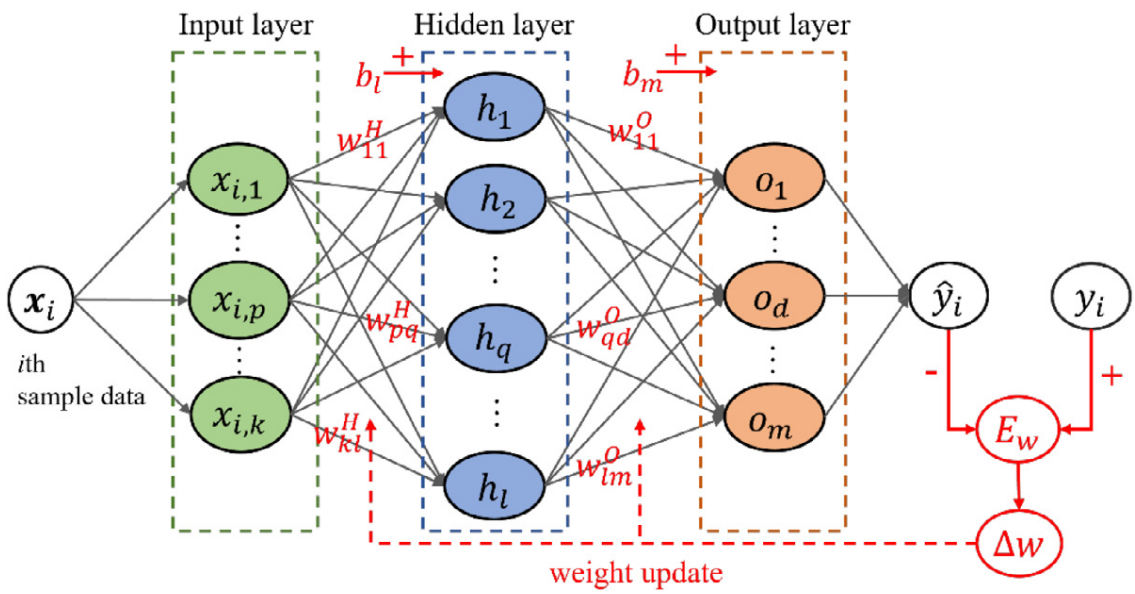
\includegraphics[width=0.6\textwidth]{chapters/chapter1/images/Figure03.png}
    \caption{The structure of the DNN \cite{ren2023review}.}
    \label{fig:figure03}
\end{figure}



\subsection{Model Training Concepts}

Effective model training ensures that neural networks learn patterns in data while minimizing errors. This section highlights essential components of the training process.

\paragraph{Loss Functions} 
Loss functions quantify the error between predicted and actual values, guiding weight updates during optimization \parencite{alzubaidi2021review}. Common loss functions include:
\begin{itemize}
    \item \textbf{Cross-Entropy Loss}: Used for classification tasks to measure the divergence between predicted probabilities and true labels.
    \item \textbf{Mean Squared Error (MSE)}: Applied in regression, computing the average squared difference between predicted and actual values.
\end{itemize}

\paragraph{Overfitting Prevention}
Overfitting occurs when a model learns noise from training data, reducing generalization to unseen data. Common techniques to mitigate overfitting include:
\begin{itemize}
    \item \textbf{Dropout}: Randomly deactivate neurons during training to enhance robustness.
    \item \textbf{Data Augmentation}: Transform training samples (e.g., rotation, scaling) to increase dataset diversity.
\end{itemize}

\paragraph{Batch Normalization}
Batch normalization stabilizes training by normalizing inputs across a mini-batch, reducing internal covariate shift and accelerating convergence.



\subsection{Optimization Methods and Strategies}
Optimization techniques in deep learning are methods used to minimize the loss function during training, improving the model’s accuracy. These techniques adjust the model's weights and biases iteratively to find the optimal set of parameters that reduces the error between predicted and actual values \parencite{alzubaidi2021review}.

Different optimizers are used to update model weights efficiently:

\begin{itemize}
    \item \textbf{Stochastic Gradient Descent (SGD):} Updates weights based on a small subset (batch) of training data, improving computational efficiency.
    \item \textbf{Adam (Adaptive Moment Estimation):} Combines momentum and adaptive learning rates for faster and more stable convergence.
    \item \textbf{RMSprop:} Uses an adaptive learning rate to prevent oscillations and improve performance on non-stationary objectives.
\end{itemize}

However, an important consideration in optimization is how to set the learning rate throughout training. While optimizers control how weights are updated, learning rate scheduling adjusts the learning rate over time to further optimize training.

Different scheduling strategies can be used in conjunction with optimizers \parencite{zhao2019learningrate}:

\begin{itemize}
    \item \textbf{Step Decay:} Reduces the learning rate at fixed intervals, allowing for more stable training as the model reaches its optimal solution.
    \item \textbf{Exponential Decay:} Gradually decreases the learning rate across epochs, promoting finer adjustments to the model parameters as the training progresses.
    \item \textbf{Cyclic Learning Rates:} Alternates between a minimum and maximum learning rate, which helps the model escape local minima and enhances exploration of the parameter space.
\end{itemize}

By combining these scheduling strategies with optimization techniques, the training process can become more efficient and effective, leading to faster and more reliable convergence.






\subsection{Model Evaluation and Validation}

Once a model is trained, it is crucial to assess its performance and ensure that it generalizes well to unseen data. This process is known as \textbf{model evaluation and validation}. The primary goal is to measure how well the model performs and to identify any potential overfitting or underfitting issues.

To evaluate a model’s performance, several metrics can be used depending on the type of task (classification, regression, etc.) \parencite{ketkar2017deep}:
\begin{itemize}
    \item \textbf{Accuracy:} For classification tasks, accuracy measures the proportion of correct predictions out of all predictions made. However, accuracy alone can be misleading in imbalanced datasets.
    \item \textbf{Precision and Recall:} In imbalanced classification problems, precision (the proportion of true positive results among all positive predictions) and recall (the proportion of true positive results among all actual positives) are often used in conjunction to provide a clearer view of the model's performance.
    \item \textbf{F1-Score:} The harmonic mean of precision and recall; F1-score balances the two metrics and is especially useful when dealing with imbalanced datasets.
    \item \textbf{Mean Squared Error (MSE):} For regression tasks, MSE calculates the average of the squared differences between predicted and actual values. It penalizes large errors more significantly than smaller ones.
    \item \textbf{R-squared (R²):} For regression, this metric indicates how well the model explains the variability in the data, with a value closer to 1 suggesting a better fit.
\end{itemize}


% \section{Deep Learning Approaches}

% Deep learning encompasses a variety of learning paradigms that enable models to extract complex patterns from large volumes of data. These approaches differ based on the nature of the data, the availability of labels, and the interaction mechanisms with the environment. This section presents the four main categories of deep learning methods \parencite{alzubaidi2021review}:

% \begin{itemize}
%     \item \textbf{Deep Supervised Learning:} This approach involves training a neural network using a labeled dataset, where each input image (e.g., leaf with visible symptoms) is paired with its correct label (e.g., disease type). The model learns to minimize the error between its predictions and the true labels using backpropagation and optimization algorithms. Techniques include Convolutional Neural Networks (CNNs) for spatial feature extraction, Deep Neural Networks (DNNs), and Recurrent Neural Networks (RNNs) like LSTMs and GRUs when dealing with sequential data.
    
%     \item \textbf{Deep Semi‐Supervised Learning:} Semi-supervised learning combines a small labeled dataset with a larger pool of unlabeled data, which is common in agricultural settings where annotating plant diseases is costly and time-consuming. Methods like Generative Adversarial Networks (GANs) can generate synthetic labeled images, while RNNs, LSTMs, and Deep Reinforcement Learning (DRL) can help model complex data behavior.
    
%     \item \textbf{Deep Unsupervised Learning:} Unsupervised learning aims to extract meaningful patterns from unlabeled data, such as grouping similar plant images or identifying features without predefined classes. Popular methods include Autoencoders for dimensionality reduction, Restricted Boltzmann Machines, and clustering algorithms. These are useful in exploratory stages or feature extraction before applying a classifier.
    
%     \item \textbf{Deep Reinforcement Learning (DRL):} In DRL, models learn optimal actions through trial and error by interacting with an environment. This could include real-time monitoring systems in agriculture, like automated disease response tools or robotic weeders. Unlike supervised learning, DRL does not require labeled data but instead uses reward signals to adjust its strategy over time.
% \end{itemize}

\section{Core Computer Vision Tasks in Agriculture}

The most common and impactful computer vision tasks include image classification, image segmentation, and object detection. Each of these tasks plays a vital role in applications such as disease diagnosis, crop monitoring, yield estimation, and weed or pest detection. The following sections explore these tasks and their corresponding deep learning techniques in detail.
\subsection{Image Classification}
Image classification is the task of assigning a label to an entire image based on its visual content. In deep learning, this is typically achieved using Convolutional Neural Networks (CNNs), which are designed to automatically learn hierarchical features from raw pixel data. 

\subsubsection{Fundamentals of CNNs}
Convolutional Neural Networks (CNNs) consist of multiple layers designed to process and learn spatial hierarchies from image data (see Figure~\ref{fig:figure04}). Their architecture typically includes \parencite{alzubaidi2021review}:

\begin{figure}[H] % 'H' needs \usepackage{float}
        \centering
        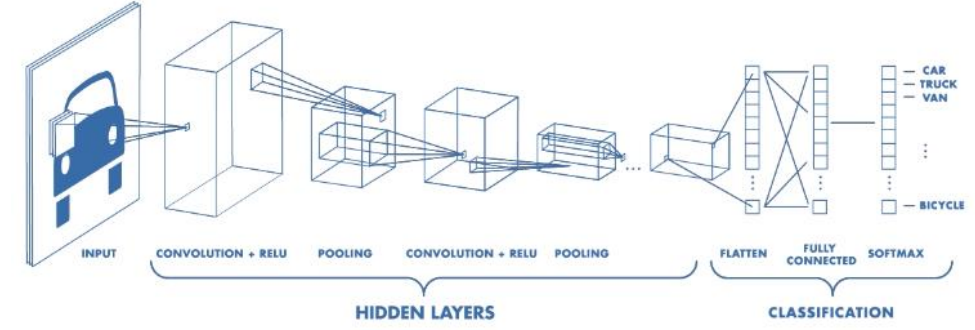
\includegraphics[width=0.9\textwidth]{chapters/chapter1/images/Figure04.png}
        \caption{Architecture of CNN \cite{purwono2022understanding}.}
        \label{fig:figure04}
    \end{figure}

\begin{itemize}
    \item \textbf{Convolutional Layers:} Extract features using small filters (kernels) that detect edges, textures, and patterns. A kernel is a grid of values (weights) initialized randomly at the start of training and adjusted through learning to identify important features.
     
     
    \begin{itemize}
        \item \textbf{Input and Kernel Dimensions:} In a CNN layer, each input $x$ is structured in three dimensions: height, width, and depth. The depth corresponds to the number of channels (e.g., an RGB image has three channels). Similarly, the kernels are also three-dimensional, with spatial dimensions (height and width) and a depth matching the input channels. Each kernel has shared parameters, a set of weights and a bias. When applied to the input, these kernels generate a corresponding set of feature maps. These kernels establish local connections by interacting only with small regions of the input at a time, allowing the network to extract patterns such as edges and textures by computing dot products across these regions.
        \item \textbf{Convolutional Operation:} The convolutional process begins by sliding the kernel across the input image in both horizontal and vertical directions. At each location, the dot product between the kernel and the overlapping region of the input is computed, producing a scalar value that becomes part of the resulting feature map. As this process is repeated across the image, a full feature map is constructed, highlighting areas where the kernel detects specific patterns. Parameters such as stride (controlling how far the kernel moves at each step) and padding (adding borders to the input to preserve edge information) affect the size and coverage of the output feature map. These concepts are illustrated in Figure~\ref{fig:figure05}.
     \end{itemize}   
    
     
    
    \begin{figure}[H] % 'H' needs \usepackage{float}
        \centering
        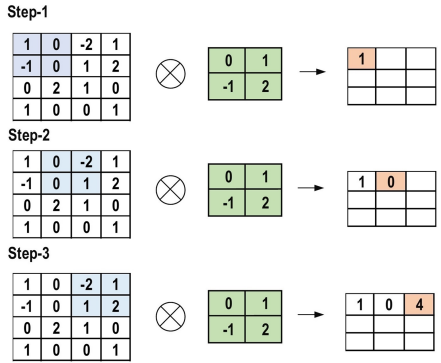
\includegraphics[width=0.6\textwidth]{chapters/chapter1/images/Figure05.png}
        \caption{The primary calculations executed at each step of the convolutional layer \parencite{alzubaidi2021review}.}
        \label{fig:figure05}
    \end{figure}

    \item \textbf{Pooling Layers:} Pooling layers are used to reduce the spatial dimensions of feature maps while preserving the most important information. This reduction helps lower the computational cost and minimizes the risk of overfitting by simplifying the data representation. The pooling operation works by sliding a small filter over the feature map and applying a summary function within each local region (Figure~\ref{fig:figure06}). Common types of pooling include:
    \begin{itemize}
        \item \textbf{Max Pooling:} Selects the maximum value in each region.
        \item \textbf{Average Pooling:} Calculates the average value of the region.
        \item \textbf{Global Average Pooling:} Computes the average across the entire feature map.
     \end{itemize}  
    
     \begin{figure}[H] % 'H' needs \usepackage{float}
        \centering
        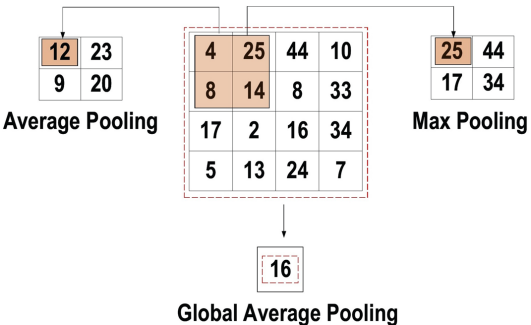
\includegraphics[width=0.6\textwidth]{chapters/chapter1/images/Figure06.png}
        \caption{Three types of pooling operations \parencite{alzubaidi2021review}.}
        \label{fig:figure06}
    \end{figure}
 
    % \item \textbf{Activation Functions:} Introduce non-linearity to help the network learn complex patterns. They must also be differentiable to enable backpropagation during training. CNNs commonly utilize the following activation functions: ReLU (Rectified Linear Unit), Sigmoid, Softmax, and Tanh.
    \item \textbf{Fully Connected Layers:} The Fully Connected (FC) layer is typically found at the end of a CNN architecture and serves as the classifier. In this layer, each neuron is connected to all neurons from the previous layer, following the fully connected approach. It operates similarly to a conventional multi-layer perceptron (MLP) network, which is a type of feed-forward artificial neural network (ANN). The input to the FC layer is a vector created from the feature maps after flattening, which comes from the last pooling or convolutional layer. The output of the FC layer represents the final result of the classification task.
    
\end{itemize}

Figure~\ref{fig:figure07} below illustrates the general structure of a Convolutional Neural Network (CNN), highlighting its layers, which work together to extract and classify features from input images.

\begin{figure}[H] % 'H' needs \usepackage{float}
    \centering
    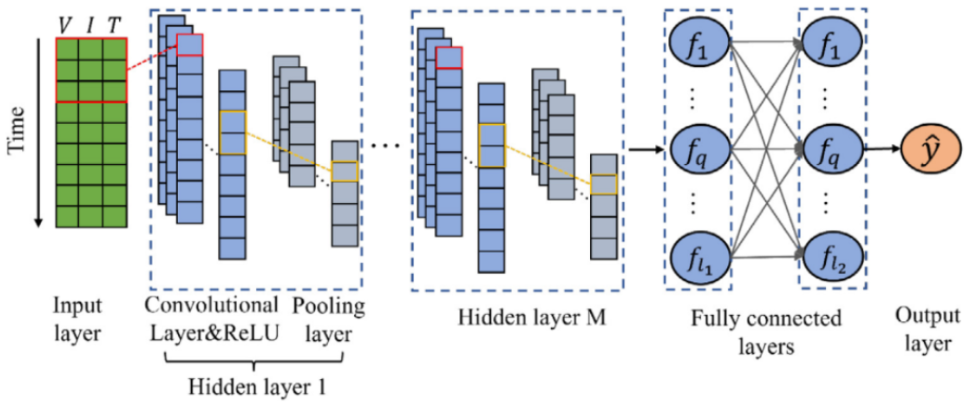
\includegraphics[width=0.9\textwidth]{chapters/chapter1/images/Figure07.png}
    \caption{The structure of the CNN \parencite{crocioni2020li}.}
    \label{fig:figure07}
\end{figure}


\subsubsection{CNN Architectures for Image Classification}
Over the past decade, numerous Convolutional Neural Network (CNN) architectures have been developed, each introducing unique design principles to improve accuracy, efficiency, and scalability. In the context of image classification, especially for tasks such as plant disease detection, the choice of architecture can significantly influence performance depending on the dataset size, complexity, and computational constraints.
This section presents an overview of some of the most influential and widely used CNN architectures:

\paragraph{Visual geometry group network (VGGNet)}
Proposed by Simonyan and Zisserman, VGGNet is a convolutional neural network (CNN) architecture widely recognized for its simplicity and strong performance in image recognition tasks.

VGG is characterized by its deep architecture, typically comprising 16 to 19 layers, which significantly enhances its representational power compared to earlier models like ZFNet and AlexNet. One of its key innovations is the replacement of large convolutional filters (such as $11 \times 11$ or $5 \times 5$) with multiple stacked $3 \times 3$ filters. This strategy maintains an equivalent receptive field while reducing the number of parameters and improving computational efficiency.

In addition, VGG uses $1 \times 1$ convolutions to control the model’s complexity and includes max pooling layers to progressively reduce the spatial dimensions of the feature maps, as illustrated in Figure~\ref{fig:figure08}.

Despite its effectiveness, a major drawback of VGGNet is its high computational cost, with around 140 million parameters \parencite{alzubaidi2021review}. Nonetheless, its reliable feature extraction capabilities have made it a popular choice in applications like plant disease classification, especially for detecting early-stage or visually subtle symptoms.


\begin{figure}[H] % 'H' needs \usepackage{float}
    \centering
    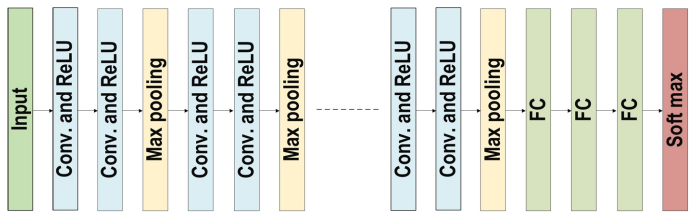
\includegraphics[width=0.8\textwidth]{chapters/chapter1/images/Figure08.png}
    \caption{The architecture of VGG \parencite{alzubaidi2021review}.}
    \label{fig:figure08}
\end{figure}

\paragraph{Inception Net (GoogLeNet)}
Inception Net, introduced by Szegedy et al., uses Inception modules that apply multiple convolutional filters ($1 \times 1$, $3 \times 3$, $5 \times 5$) in parallel, followed by concatenation (see Figure~\ref{fig:figure09}). This design captures multi-scale information efficiently while reducing computational cost. The architecture has been successfully applied in plant phenotyping and classification of complex disease patterns.

It replaced standard convolutional layers with micro-neural networks and regulated computation through $1 \times 1$ convolutions as bottleneck layers. Sparse connections addressed redundant information by selectively connecting input and output channels, while the global average pooling (GAP) layer reduced parameters from 40 million to just 5 million, enhancing efficiency. Additional features included the RmsProp optimizer, batch normalization, and auxiliary learners to accelerate convergence \parencite{alzubaidi2021review}.



\begin{figure}[H] % 'H' needs \usepackage{float}
    \centering
    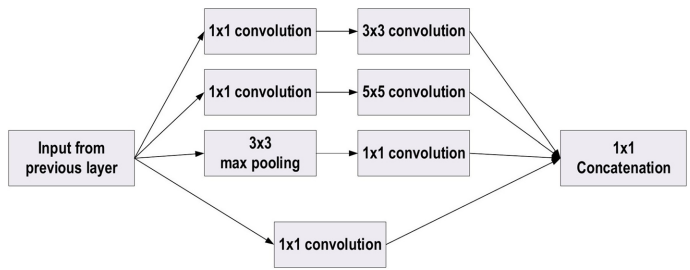
\includegraphics[width=0.8\textwidth]{chapters/chapter1/images/Figure09.png}
    \caption{The basic structure of Google Block \parencite{alzubaidi2021review}.}
    \label{fig:figure09}
\end{figure}

\paragraph{Xception Net}

The Xception model is an extension of the Inception architecture that replaces standard convolutions with depth-wise separable convolutions, significantly improving efficiency. It has been shown to outperform Inception in many tasks, especially with high-resolution agricultural images, by learning spatial and cross-channel correlations separately.

The core concept behind Xception is the modification of the traditional Inception block by making it wider and replacing the standard $3 \times 3$ convolution followed by a $1 \times 1$ convolution with depthwise separable convolutions, which reduces computational complexity while enhancing performance \parencite{alzubaidi2021review}. An illustration of the basic Xception block structure is presented in Figure~\ref{fig:figure10}.


\begin{figure}[H] % 'H' needs \usepackage{float}
    \centering
    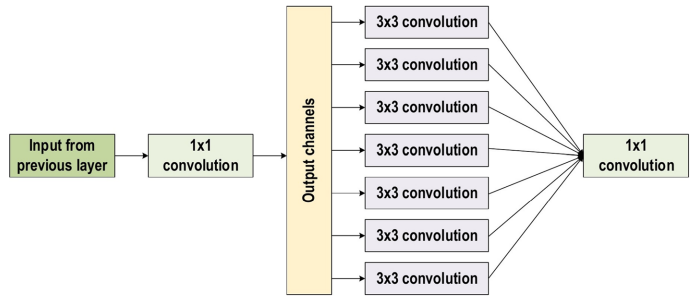
\includegraphics[width=0.8\textwidth]{chapters/chapter1/images/Figure10.png}
    \caption{The basic block diagram for the Xception block architecture \parencite{alzubaidi2021review}.}
    \label{fig:figure10}
\end{figure}

\paragraph{Residual Networks (ResNet)}
ResNet is a deep convolutional neural network architecture developed to facilitate the training of very deep networks, ranging from 18 to 152 layers, by introducing the concept of residual learning through shortcut (or skip) connections that bypass one or more layers.

These residual connections address the degradation problem that often occurs in deeper networks, where increasing depth leads to performance saturation or even degradation. By enabling gradients to flow more efficiently, ResNet makes it easier for the network to learn identity mappings or residual functions, simplifying the overall training process.

The output of a residual block is defined as:
\begin{equation}
    H(x) = F(x) + x  \tag{3}
\end{equation}

Where:
\begin{itemize}
    \item $H(x)$: the output of the residual block,
    \item $F(x)$: the residual function to be learned,
    \item $x$: the input passed through the shortcut connection.
\end{itemize}

This formulation (3) makes it easier to optimize deep networks by learning the difference (residual) between the desired mapping and the identity. Additionally, it helps increase the rank of the weight matrices, enhancing the network’s expressiveness and preventing performance degradation.

An illustration of the residual module structure is provided in Figure~\ref{fig:figure11}.


\begin{figure}[H] % 'H' needs \usepackage{float}
    \centering
    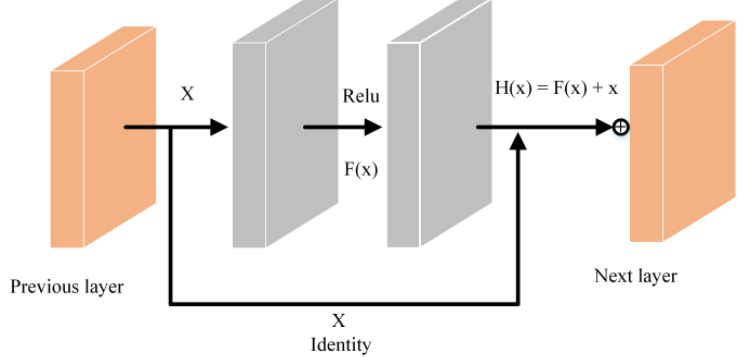
\includegraphics[width=0.6\textwidth]{chapters/chapter1/images/Figure11.png}
    \caption{Residual module diagram \parencite{fang2023lightweight}.}
    \label{fig:figure11}
\end{figure}

% \subsubsection{DenseNet}

% DenseNet is a convolutional neural network architecture that introduces the concept of dense connectivity, in which each layer is directly connected to every other layer in a feed-forward fashion, as illustrated in Figure~\ref{fig:figure12}. This unique design enables feature reuse, enhances gradient flow, and significantly reduces the number of parameters compared to traditional CNNs.

% Inspired by ResNet and Highway Networks, DenseNet addresses a key limitation in ResNet, where each layer maintains isolated weights and where certain transformations contribute minimal new information. In contrast, DenseNet concatenates the outputs of all preceding layers and feeds them as input to each subsequent layer.

% In a DenseNet with $l$ layers, the number of direct connections between layers is given by:
% \[
% \text{Number of connections} = \frac{l(l+1)}{2} \tag{4}
% \]

% This connectivity pattern facilitates richer feature propagation, introduces a regularization effect, and helps mitigate the vanishing gradient problem, thus improving training efficiency and model generalization \parencite{alzubaidi2021review}.

% Despite the computational cost introduced by the accumulation of feature maps, DenseNet has shown exceptional performance in fine-grained classification tasks, such as distinguishing between subtly different plant disease symptoms, particularly in scenarios with limited training data.

% \begin{figure}[H] % 'H' needs \usepackage{float}
%     \centering
%     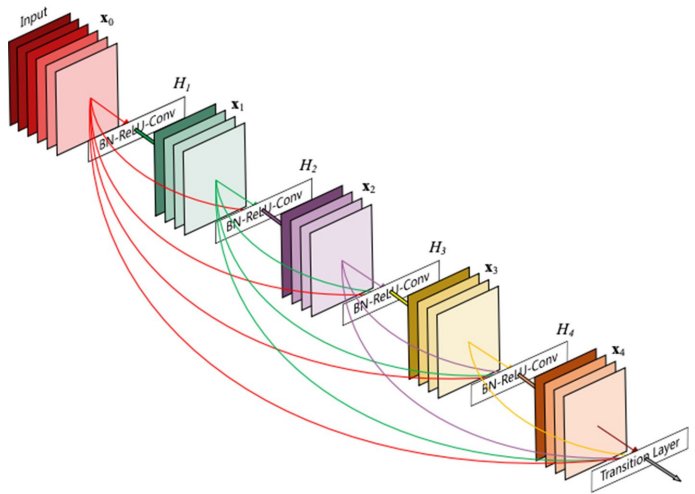
\includegraphics[width=0.6\textwidth]{chapters/chapter1/images/Figure12.png}
%     \caption{The architecture of DenseNet Network \parencite{alzubaidi2021review}.}
%     \label{fig:figure12}
% \end{figure}


% \subsubsection{EfficientNet}


% EfficientNet is a family of convolutional neural networks developed by Google AI that introduces a compound scaling method to efficiently scale deep learning models. Traditional approaches often scale models arbitrarily in one of three dimensions: depth (number of layers), width (number of channels), or input resolution. However, EfficientNet proposes a more balanced and systematic strategy, where all three dimensions are scaled simultaneously and proportionally using a fixed set of scaling coefficients. This compound approach maintains model efficiency while significantly boosting accuracy.

% The baseline model, EfficientNet-B0 (see Figure~\ref{fig:figure13}), is built using Neural Architecture Search (NAS) to optimize both performance and efficiency. Larger variants (B1 to B7) are derived by uniformly scaling the baseline model using the compound scaling principle. This results in models that achieve state-of-the-art performance on image classification tasks with dramatically fewer parameters and lower computational cost compared to earlier architectures like ResNet or Inception.

% \begin{figure}[H] % 'H' needs \usepackage{float}
%     \centering
%     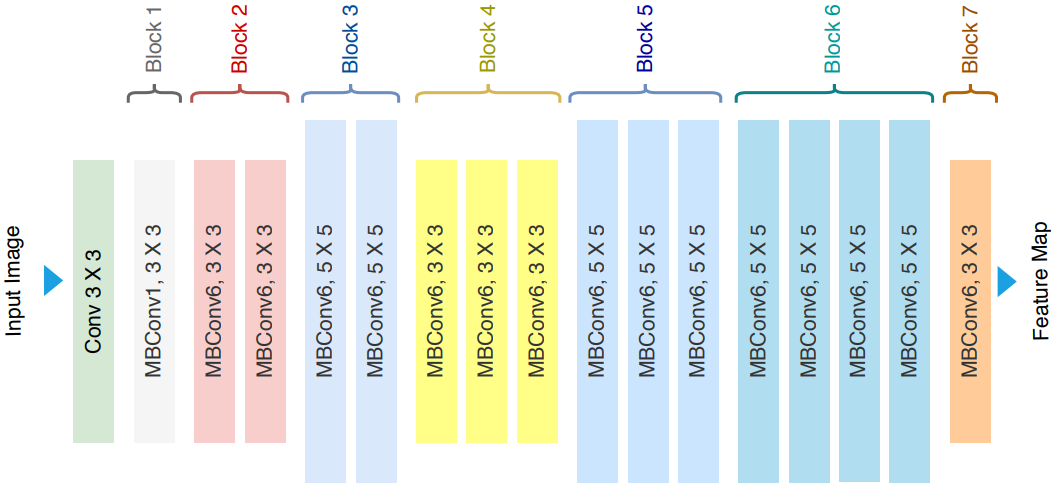
\includegraphics[width=0.6\textwidth]{chapters/chapter1/images/Figure13.png}
%     \caption{Architecture of EfficientNet-B0 with MBConv as Basic building blocks \parencite{ahmed2022classification}.}
%     \label{fig:figure13}
% \end{figure}

\paragraph{Lightweight and Specialized CNN Models}
Several CNN architectures, such as MobileNet, EfficentNet, and ShuffleNet, have been specifically developed to meet constraints related to speed, model size, and power efficiency, making them suitable for deployment on mobile or edge devices. Although not explored in depth within the main text, a comparative overview of their architectures, key characteristics, and potential applications in smart agriculture is presented in Appendix\ref{app:annexA} for further reference.


\subsubsection{Transfer Learning and Pretrained Models}
% In deep learning, training models from scratch often requires large labeled datasets and significant computational resources. Transfer learning offers a powerful alternative by leveraging models pre-trained on large benchmark datasets such as \textbf{ImageNet}. These pre-trained models capture rich and generalizable features in their initial layers, which can then be adapted to new, often smaller, target datasets with minimal additional training.
% This section explores the concept of transfer learning, introduces popular pre-trained CNN architectures relevant to agricultural applications, and outlines fine-tuning strategies suitable for small-scale plant datasets.

% \subsection{Concept of Transfer Learning}
Transfer learning is a machine learning technique where a model trained on one task is repurposed for a different but related task. In the context of deep learning, it typically involves taking a neural network pre-trained on a large dataset such as ImageNet, which contains over 14 million labeled images, and adapting it to a specific task that may lack sufficient labeled data.

To formalize this, consider a target learning task \( T_t \) based on a domain \( D_t \); transfer learning allows for assistance from a different domain \( D_s \) for the learning task \( T_s \). The goal of transfer learning is to improve the performance of the predictive function \( f_{T_t}(\cdot) \) for the task \( T_t \) by discovering and transferring latent knowledge from \( D_s \) and \( T_s \), where generally \( D_s = D_t \) and/or \( T_s = T_t \). Furthermore, it is often the case that the size of \( D_s \) is much larger than that of \( D_t \) \parencite{tan2018survey}.

This process is illustrated in Figure~\ref{fig:figure14}, which demonstrates how knowledge from a source task and domain can be transferred to a target task with limited data.

\begin{figure}[H] % 'H' needs \usepackage{float}
    \centering
    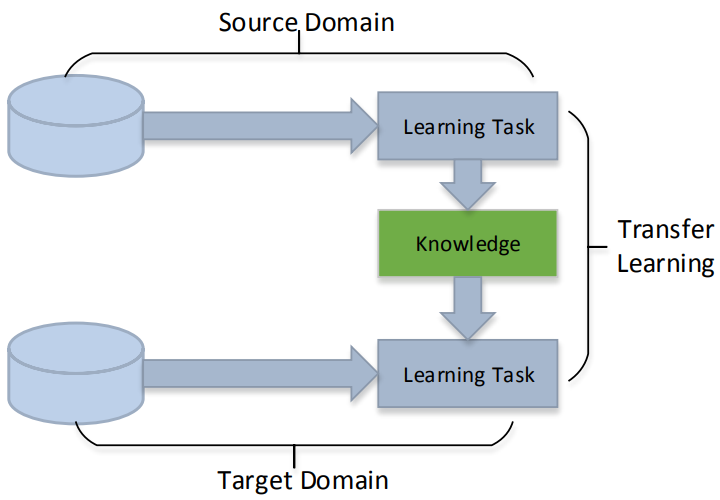
\includegraphics[width=0.5\textwidth]{chapters/chapter1/images/Figure14.png}
    \caption{Learning process of transfer learning \parencite{tan2018survey}.}
    \label{fig:figure14}
\end{figure}
The two primary approaches to transfer learning are \parencite{tan2018survey}:

\begin{itemize}
    \item \textbf{Feature Extraction:} The pre-trained model is used as a fixed feature extractor. All convolutional layers are kept frozen, and only the final fully connected layer(s) are trained on the new dataset.
    \item \textbf{Fine-Tuning:} Some layers of the pretrained model are unfrozen and retrained on the new dataset. This allows the model to slightly adjust its learned features to better suit the new domain.
\end{itemize}

% This concept is illustrated in Figure~\ref{fig:figure15}, which demonstrates the integration of a custom CNN with transfer learning networks.

% \begin{figure}[H] % 'H' needs \usepackage{float}
%     \centering
%     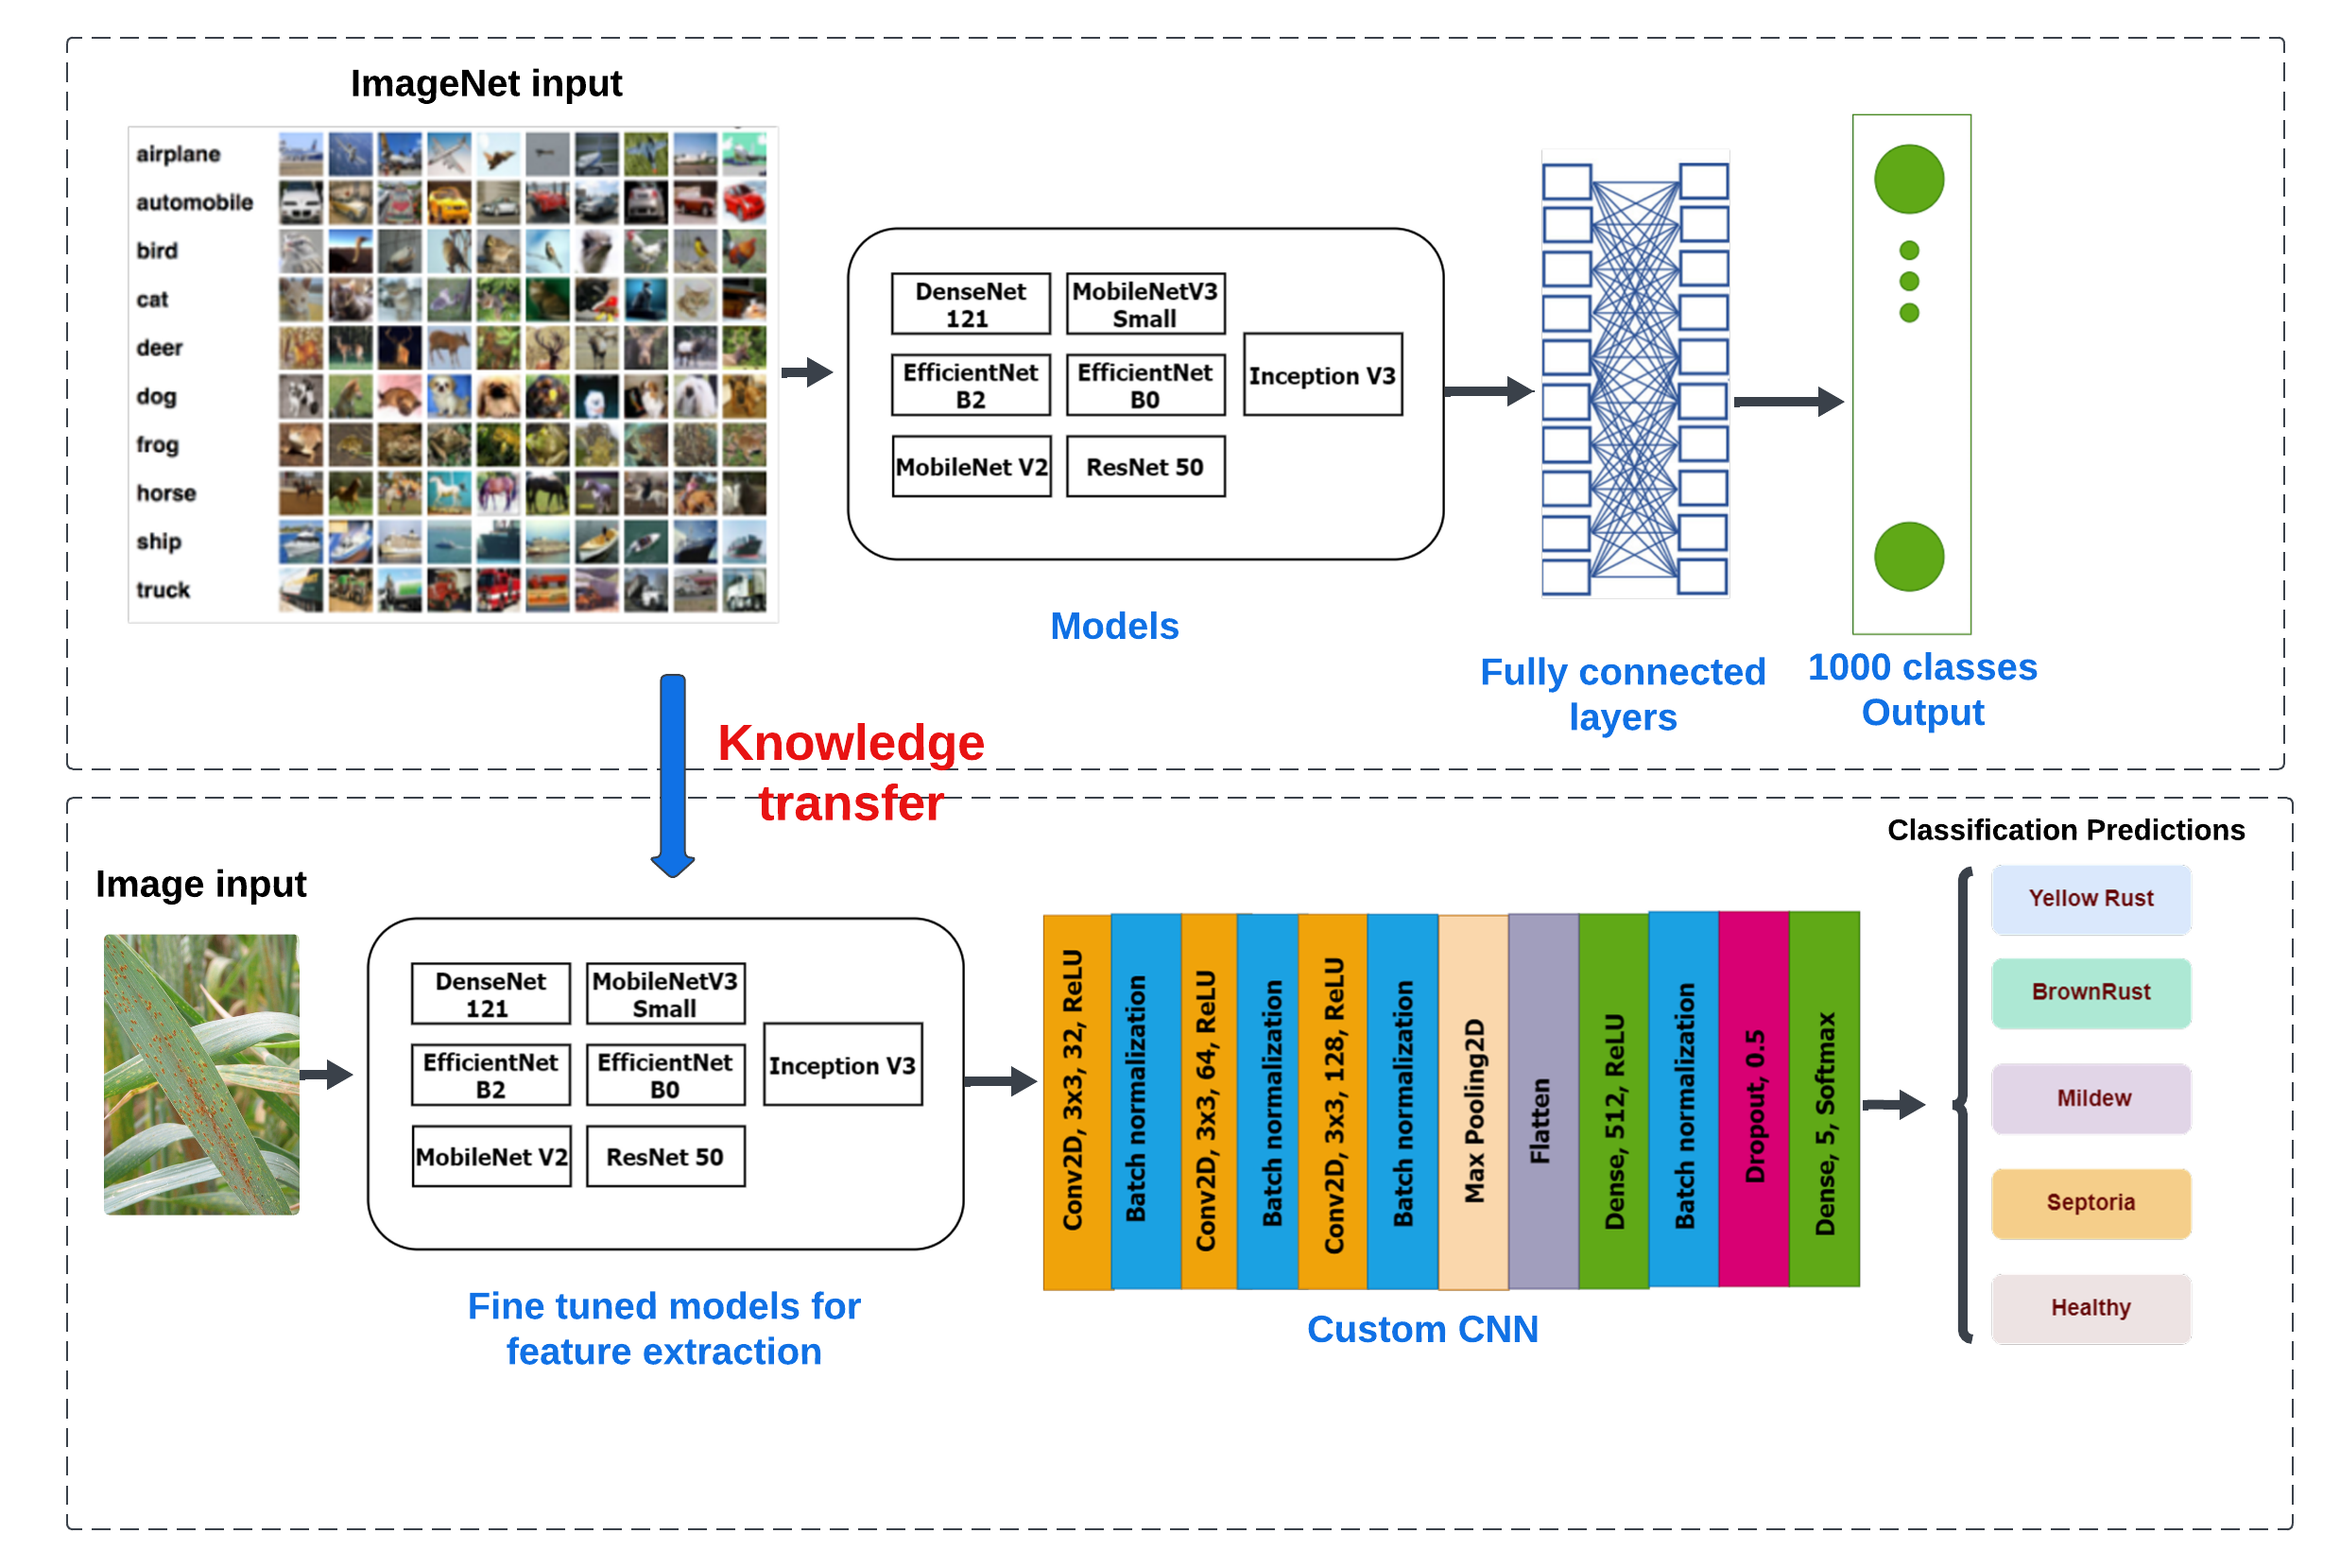
\includegraphics[width=0.8\textwidth]{chapters/chapter1/images/Figure15.png}
%     \caption{Integration of the custom CNN with transfer learning networks \parencite{jouini2024wheat}.}
%     \label{fig:figure15}
% \end{figure}

% Transfer learning is especially valuable in agriculture, where acquiring large annotated datasets is difficult. By leveraging pre-trained models, researchers and practitioners can build effective models for plant disease detection with limited data and reduced computational cost


% \subsection{Fine-Tuning Strategies for Agricultural Data}


% While basic fine-tuning involves unfreezing and retraining a subset of layers in a pretrained model, fine-tuning strategies can be further optimized when dealing with agricultural data, which often presents unique challenges such as class imbalance, limited samples, and high intra-class variability (e.g., similar symptoms across different plant diseases). 

% In this context, several fine-tuning strategies can be applied to improve model generalization and performance:
% \begin{itemize}
%     \item \textbf{Gradual Unfreezing:} Instead of unfreezing all layers at once, layers are incrementally unfrozen, starting from the top (fully connected layers) and moving backward. This helps prevent the model from losing previously learned useful features during early training stages \parencite{hossen2025transfer}.
%     \item \textbf{Discriminative Learning Rates:} Assigning different learning rates to different layers, lower for earlier layers and higher for later ones, ensures that the more generic features are preserved while higher-level representations are fine-tuned for the new task \parencite{hossen2025transfer}.
%     \item \textbf{Early Stopping and Regularization:} Due to limited data, it's essential to prevent overfitting during fine-tuning. Techniques like early stopping, dropout, and weight decay can help maintain model robustness \parencite{li2021implicit}.
%     \item \textbf{Data Augmentation and Balancing:} Supplementing fine-tuning with targeted data augmentation (e.g., rotation, brightness adjustments, zoom) helps the model generalize better. In addition, synthetic oversampling techniques like SMOTE can address class imbalance issues \parencite{aquino2017effect}.
% \end{itemize}

% These strategies, when integrated thoughtfully, allow researchers to tailor fine-tuning to the specific nature of agricultural datasets, maximizing the benefits of transfer learning even in data-constrained environments.


\subsection{Object Detection}
In the context of precision agriculture, object detection has emerged as a critical computer vision technique for automating the assessment of crop health. It facilitates the identification and localization of plant diseases, nutrient deficiencies, and weeds, supporting more efficient and timely interventions across large-scale farming environments. 

At its core, object detection involves predicting both the category and precise location of objects within an image, thus combining classification with localization. Traditional approaches consist of stages such as region proposal, feature extraction, and object classification. Over time, detection methods have evolved to address increasing demands for accuracy and speed, giving rise to both two-stage and one-stage detection frameworks \parencite{zhao2019objectdetection}.

Here are more details about the concepts of object detection \parencite{zhao2019objectdetection}: 
\begin{itemize}
    \item \textbf{Informative Region Selection:} It is used to identify specific areas within an image where objects are likely to appear. This step helps reduce computational load by focusing only on promising regions instead of scanning the entire image at all scales and positions. In agricultural imagery, objects like plants or pests may vary in size, shape, and location. Early methods used multiscale sliding windows to generate candidate regions, but this approach was computationally expensive and often produced redundant proposals. To improve efficiency, modern techniques now use region proposal algorithms or attention mechanisms to better focus on meaningful areas while avoiding irrelevant ones.
    \item \textbf{Feature Extraction:} It is the process of identifying and isolating relevant visual attributes from an image that can effectively represent objects within it. Object recognition involves detecting characteristics that are both robust and semantically significant. Traditional methods such as Scale-Invariant Feature Transform (SIFT), Histograms of Oriented Gradients (HOG), and Haar-like features were designed to mimic human vision by emphasizing edges, textures, and patterns. However, these handcrafted techniques often struggled to maintain performance due to challenges like changes in object appearance, lighting variations, and cluttered backgrounds, leading to their limitations in complex scenarios.
    \item \textbf{Classification and Localization:} Classification and localization refer to the process of both identifying the object in an image and determining its precise location through bounding boxes. With the rise of deep learning, this step underwent a significant transformation. Models such as R-CNN and its subsequent versions: Fast R-CNN, Faster R-CNN, and YOLO (You Only Look Once)automated the feature extraction process and seamlessly integrated classification with bounding box regression. These advancements led to substantial improvements in both detection accuracy and processing speed, enabling real-time applications in fields like crop monitoring and pest detection.
\end{itemize}

\subsubsection{Annotation of Objects}
Annotation refers to the process of labeling the objects (such as pests, diseases, or damaged crops) in the images by drawing bounding boxes around them and assigning class labels. This is a critical step for supervised learning, where the model learns to identify patterns based on labeled data. Several annotation techniques can be used:
\begin{itemize}
    \item \textbf{Bounding Boxes:} The most common annotation method in object detection. Each object is enclosed in a rectangular box, and the class of the object is assigned to it (e.g., "rust", "aphid").
    \item \textbf{Polygons:} For more precise object delineation, especially when objects have irregular shapes (e.g., plant leaves affected by disease), polygons are used instead of bounding boxes.
    % \item \textbf{Semantic Segmentation:} In cases where the task involves classifying each pixel in the image, semantic segmentation labels each pixel to indicate which class it belongs to (e.g., diseased or healthy tissue in a leaf).
\end{itemize}

\subsubsection{Evaluation Metrics in Object Detection}    
In object detection, several metrics are used to assess model performance:
\begin{itemize}
    \item \textbf{Mean Average Precision (mAP):} Measures the average precision across all object classes, balancing precision and recall to evaluate overall model performance.
    \item \textbf{Intersection over Union (IoU):} Calculates the overlap between predicted and ground truth bounding boxes, indicating localization accuracy. Higher IoU means better localization.
    
    \item \textbf{Precision:} Measures the proportion of true positive detections out of all predicted objects.
    \item \textbf{Recall:} Measures the proportion of true positive detections out of all actual objects.
   
    \item \textbf{F1-Score:} The harmonic mean of precision and recall, providing a balance between both.
    \item \textbf{Average Recall (AR):} Evaluates recall at different IoU thresholds, useful for detecting small objects or handling occlusions.
    \item \textbf{Confusion Matrix:} Summarizes true positives, false positives, true negatives, and false negatives, providing insights into model errors.
    \item \textbf{Speed Metrics (FPS, Latency):} Assess real-time performance, essential for time-sensitive applications like precision agriculture.
    \item \textbf{AP at Specific IoU Thresholds:} Measures precision at different IoU levels to understand performance under stricter conditions.
\end{itemize}

\subsubsection{Key Architectures}
Many architectures are designed to efficiently and accurately detect objects in images, even in complex agricultural environments. Below, we discuss four of the most widely used and effective object detection models: YOLO (You Only Look Once), R-CNN, and SSD (Single Shot Multibox Detector). 

\subsubsection{Yolo}
YOLO is a fast and efficient object detection framework that predicts both object confidences and bounding boxes (BBs) using the entire topmost feature map. The image is divided into a $S \times S$ grid, where each grid cell is responsible for predicting objects centered within it. Each cell predicts multiple bounding boxes and their corresponding confidence scores, which reflect the likelihood of an object being present and how well the predicted box overlaps with the ground truth (IoU) (see figure~\ref{fig:figure16}).

At test time, class-specific confidence scores are computed by multiplying the box confidence with conditional class probabilities. YOLO optimizes a loss function during training to fine-tune predictions and improve detection accuracy \parencite{zhao2019objectdetection}.

\begin{figure}[H] % 'H' needs \usepackage{float}
    \centering
    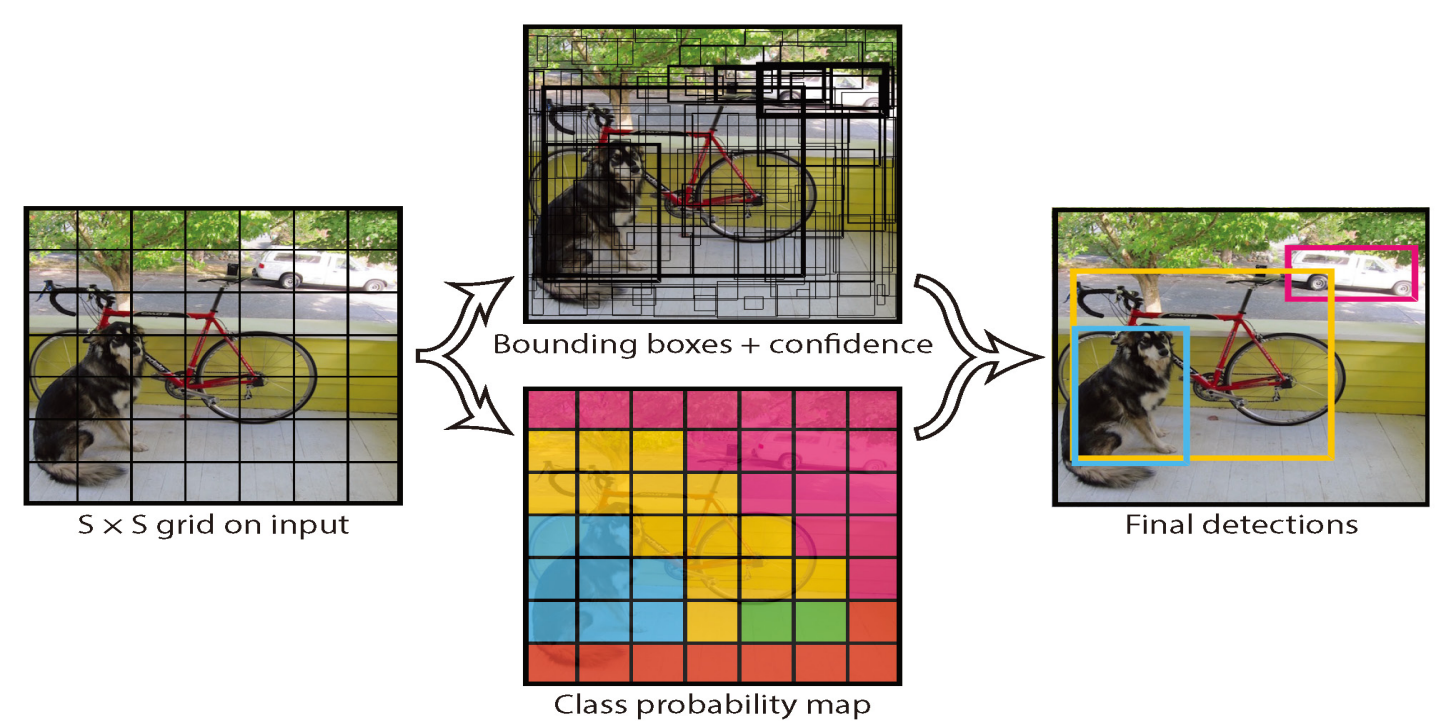
\includegraphics[width=0.8\textwidth]{chapters/chapter1/images/Figure16.png}
    \caption{Main idea of YOLO \parencite{zhao2019objectdetection}.}
    \label{fig:figure16}
\end{figure}

\subsubsection{R-CNN}
R-CNN is a significant advancement in object detection, improving the quality of candidate bounding boxes (BBs) and utilizing deep architecture for high-level feature extraction \parencite{zhao2019objectdetection}. It consists of three main stages, as presented in figure~\ref{fig:figure17}:

\begin{itemize}
    \item \textbf{Region Proposal Generation:} R-CNN uses selective search to generate about 2000 region proposals per image, improving candidate box accuracy and reducing the search space.
    \item \textbf{CNN-Based Feature Extraction:} Each region proposal is resized and passed through a CNN to extract a 4096-dimensional feature, creating a high-level, robust representation of the object.
    \item \textbf{Classification and Localization:} Region proposals are classified using pre-trained linear SVMs, and bounding box regression is applied. Non-maximum suppression (NMS) is used to eliminate redundant boxes and finalize object detections.
\end{itemize}

\begin{figure}[H] % 'H' needs \usepackage{float}
    \centering
    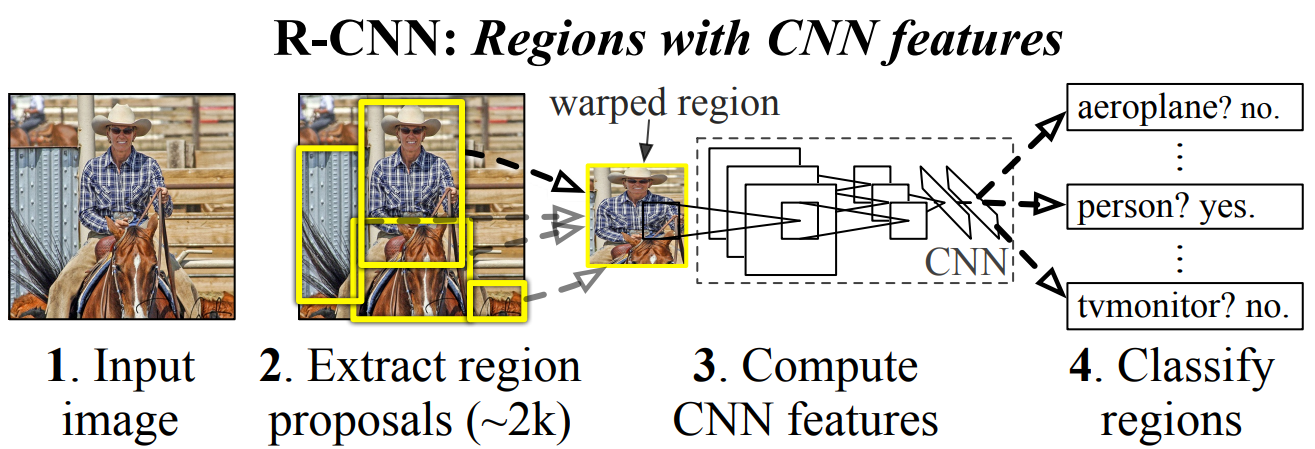
\includegraphics[width=0.7\textwidth]{chapters/chapter1/images/Figure17.png}
    \caption{Flowchart of R-CNN \parencite{zhao2019objectdetection}.}
    \label{fig:figure17}
\end{figure}

Despite its success, R-CNN has drawbacks, including slow inference due to CNN computation for each region, time-consuming multistage training, high memory and storage requirements for storing region features, and redundant region proposals from selective search that slow down the process \parencite{zhao2019objectdetection}.


% \paragraph{Faster R-CNN}


% Faster R-CNN improves upon earlier object detection models by introducing a Region Proposal Network (RPN), a deep learning-based method for generating object proposals, which shares convolutional features with the detection network to generate object proposals efficiently, eliminating the need for methods like selective search. The RPN uses a fully convolutional network (FCN) (as presented in Figure~\ref{fig:figure18}) to predict bounding boxes and object scores simultaneously. The system uses anchors of multiple scales and aspect ratios and is trained end-to-end with a multitask loss function. While Faster R-CNN achieves state-of-the-art accuracy and high-speed processing, it is limited by its alternate training algorithm, which is time-consuming and struggles with extreme object scales and shapes \parencite{zhao2019objectdetection}.

% \begin{figure}[H] % 'H' needs \usepackage{float}
%     \centering
%     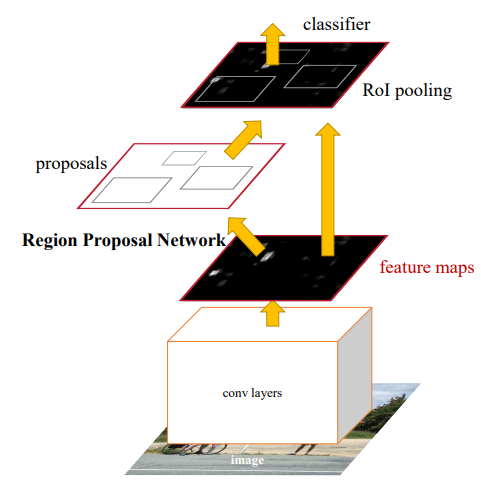
\includegraphics[width=0.6\textwidth]{chapters/chapter1/images/Figure18.png}
%     \caption{An illustration of the Faster R-CNN model \parencite{ren2016faster}.}
%     \label{fig:figure18}
% \end{figure}

\subsubsection{SSD}
SSD was introduced to address the limitations of YOLO, particularly in handling small objects and objects with unusual aspect ratios. Unlike YOLO's fixed grid approach, SSD uses default anchor boxes of various aspect ratios and scales to better handle objects of different sizes.

It integrates predictions from multiple feature maps with different resolutions and uses a VGG16 backbone architecture with additional layers for bounding box predictions. SSD is trained with a combination of localization and confidence losses and refines detections using non-maximum suppression (NMS). It outperforms Faster R-CNN in accuracy on PASCAL VOC and COCO while being three times faster, running at 59 fps with an input size of 300 × 300. However, SSD still struggles with small objects, which can be improved with better feature extractors and network modifications \parencite{zhao2019objectdetection}.

Below is the architecture of SSD (Figure~\ref{fig:figure19}), illustrating its key components, including the VGG-16 backbone, extra feature layers, and classifier convolutions.

\begin{figure}[H] % 'H' needs \usepackage{float}
    \centering
    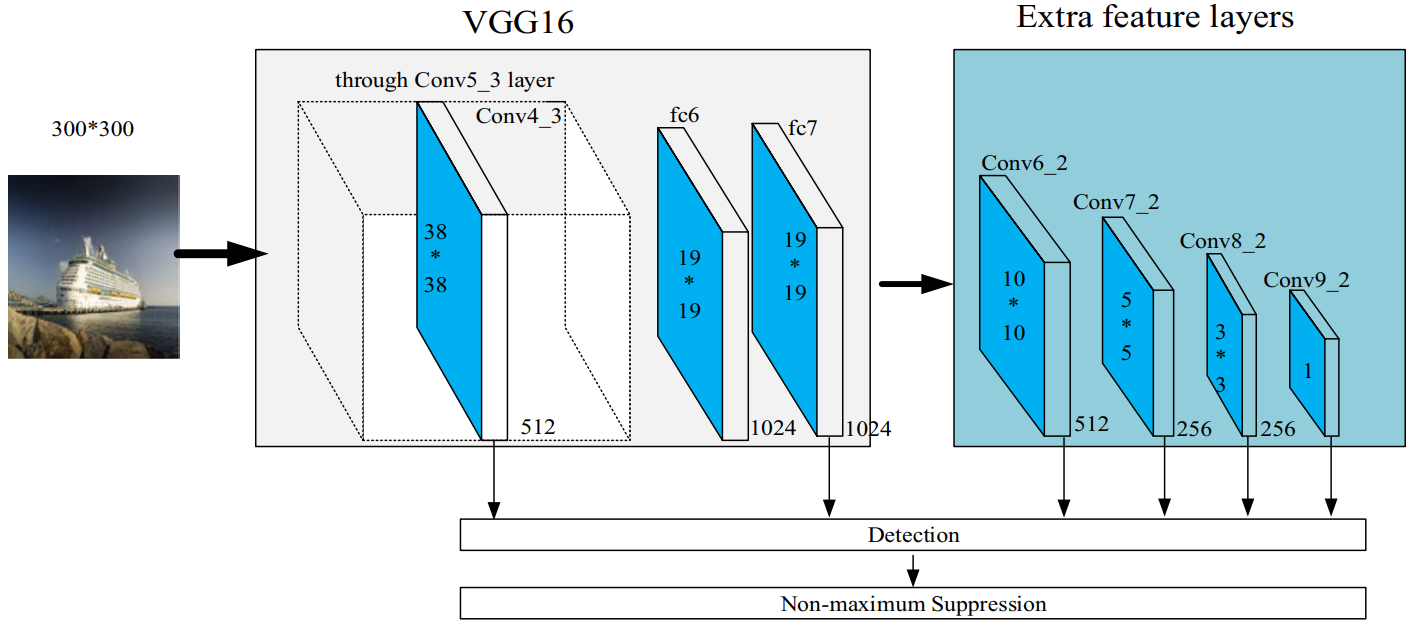
\includegraphics[width=0.8\textwidth]{chapters/chapter1/images/Figure19.png}
    \caption{Architecture of SSD \parencite{li2021water}.}
    \label{fig:figure19}
\end{figure}

\subsection{Image Segmentation}
Image segmentation is a computer vision task that involves partitioning an image into multiple segments, or regions, to make the analysis of its content more manageable. Each pixel is classified into a specific category, which helps in identifying objects or boundaries within an image. In wheat disease detection, image segmentation is crucial for isolating affected areas and distinguishing between healthy and diseased plant tissues. Models like PSPNet, U-Net and its variants, and DeepLabV3+ are particularly effective for this task, as they can capture both fine details and global context, leading to more accurate disease detection.

\subsubsection{Pyramid Scene Parsing Network (PSPNet)}
Pyramid Scene Parsing Network (PSPNet) is a deep convolutional neural network architecture designed for semantic segmentation tasks, particularly effective in capturing both local and global contextual information. The core innovation of PSPNet lies in its Pyramid Pooling Module (PPM), which aggregates context from different regions of the image at multiple scales. This is achieved by applying pooling operations at varying grid sizes, then upsampling and concatenating these pooled features with the original feature maps \parencite{pan2021deep}. This fusion allows PSPNet to understand the spatial hierarchy and global structure of scenes more effectively than traditional CNNs (Figure~\ref{fig:PSPNet}). ResNet and its variants are usually used as the backbone for PSPNet due to their residual (skip) connections, which help alleviate the vanishing gradient problem and enable effective training of deep networks, making them well-suited for extracting rich feature representations in segmentation tasks.
\begin{figure}[H] % 'H' needs \usepackage{float}
    \centering
    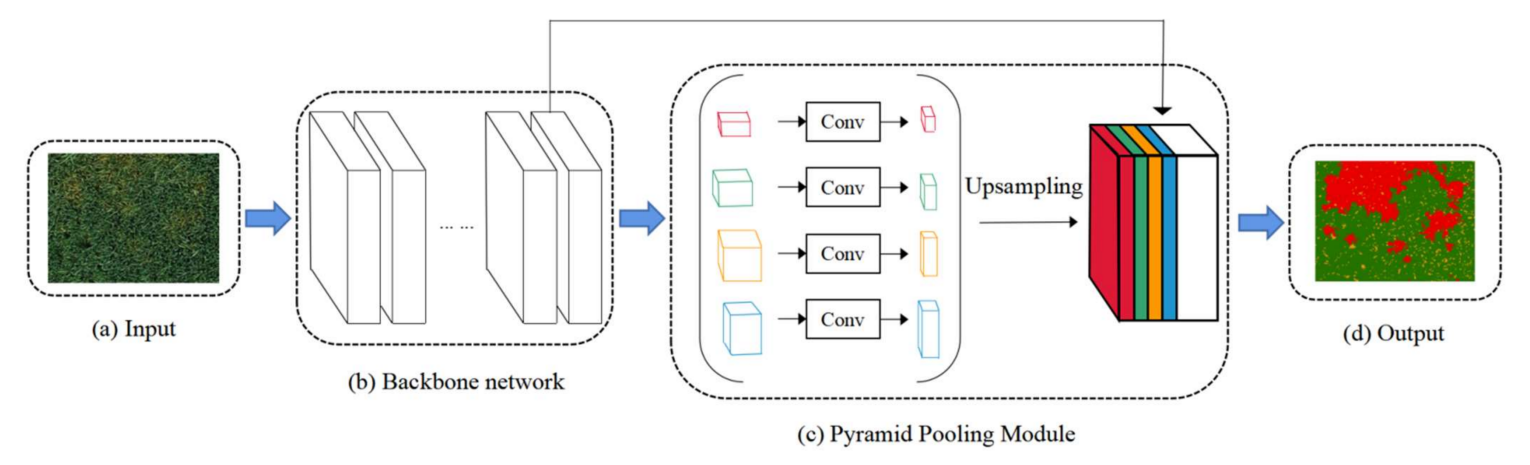
\includegraphics[width=0.9\textwidth]{chapters/chapter1/images/Figure20.png}
    \caption{Semantic Segmentation of Wheat Yellow Rust Using PSPNet \parencite{pan2021deep}.}
    \label{fig:PSPNet}
\end{figure}

\subsubsection{U-Net Model Architecture}
U-Net is a convolutional neural network architecture designed for semantic segmentation, featuring a symmetric encoder-decoder structure. The encoder, or contracting path, captures contextual features using repeated 3×3 convolutions with ReLU activation, followed by 2×2 max pooling for downsampling. The decoder, or expansive path, performs upsampling and applies 3×3 convolutions to recover spatial resolution. Crucially, skip connections between corresponding encoder and decoder layers preserve high-resolution features, improving segmentation accuracy. A final 1×1 convolution maps the feature maps to the desired number of output classes. All convolutions use "same" padding with stride [1,1], and max pooling uses stride [2,2] with zero padding. ReLU activation is applied throughout the network, and input images undergo zero-center normalization for training stability \parencite{su2020aerial}. This architectural layout, including feature map sizes and layer depths, is depicted in Figure~\ref{fig:U-Net}.
\begin{figure}[H] % 'H' needs \usepackage{float}
    \centering
    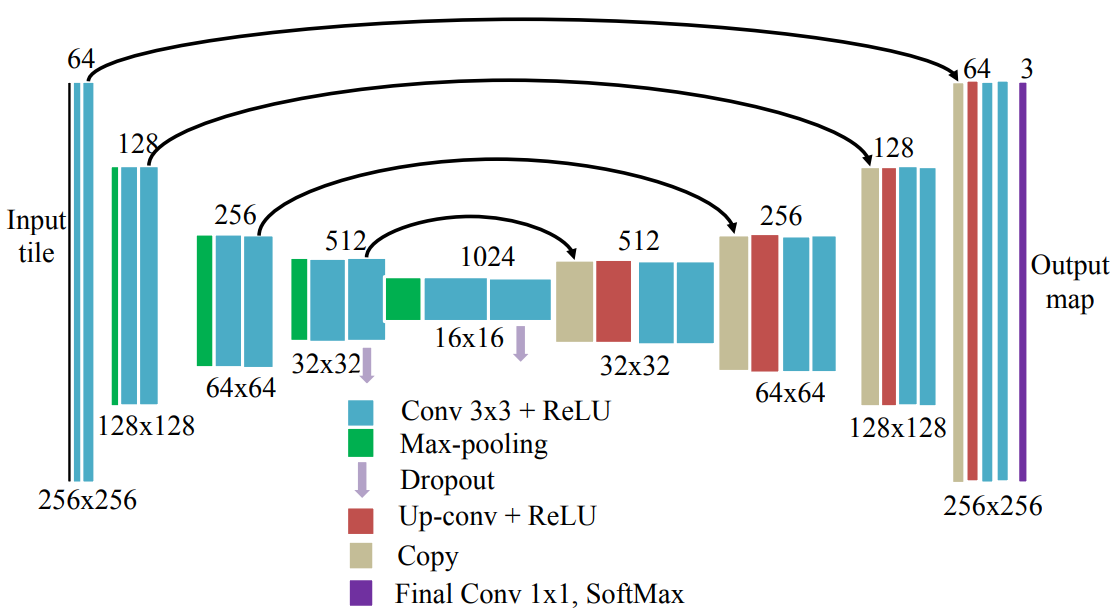
\includegraphics[width=0.6\textwidth]{chapters/chapter1/images/Figure21.png}
    \caption{U-Net Architecture for Semantic Segmentation \parencite{su2020aerial}.}
    \label{fig:U-Net}
\end{figure}
Several U-Net variants have been proposed to address computational efficiency and feature enhancement:
\begin{itemize}
    \item \textbf{LR-UNet (Lightweight Residual U-Net)}: This architecture introduces residual connections and lightweight convolutional blocks to reduce the number of parameters and computational cost while maintaining segmentation performance. It is especially suitable for deployment in resource-constrained environments such as mobile or embedded devices \parencite{zhang2021irunet}.
    
    \item \textbf{DF-UNet (Dual Feature U-Net)}: This model enhances the original U-Net by fusing both shallow (low-level spatial) and deep (high-level semantic) features. This dual feature strategy improves the network's ability to detect fine edges and preserve structural details, particularly in complex segmentation tasks such as medical or remote sensing imagery. DF-UNet may also integrate attention mechanisms and refined skip connections for more effective feature reuse \parencite{zhang2022wheat}.
\end{itemize}

\subsubsection{DeepLabV3+}
DeepLabV3+ is an advanced semantic segmentation model that builds upon DeepLabV3 by combining powerful contextual feature extraction with precise boundary recovery. DeepLabV3 uses Atrous Spatial Pyramid Pooling (ASPP) to capture multi-scale contextual information through parallel atrous (dilated) convolutions with varying rates, allowing the model to extract rich semantic features without reducing spatial resolution too much. However, DeepLabV3 lacks a decoder and relies on simple bilinear upsampling, which limits its ability to recover fine object boundaries. DeepLabV3+ (Figure~\ref{fig:DeepLabv3+}) addresses this by introducing a decoder module that refines segmentation results, especially along object edges, by upsampling the encoder’s output and combining it with low-level features from earlier layers of the network, followed by a few convolutions for detail refinement. Additionally, DeepLabV3+ applies depthwise separable (atrous separable) convolutions in both the ASPP and decoder modules to reduce computational cost while maintaining high accuracy, resulting in a more accurate and efficient architecture \parencite{chen2018encoder}.
\begin{figure}[H] % 'H' needs \usepackage{float}
    \centering
    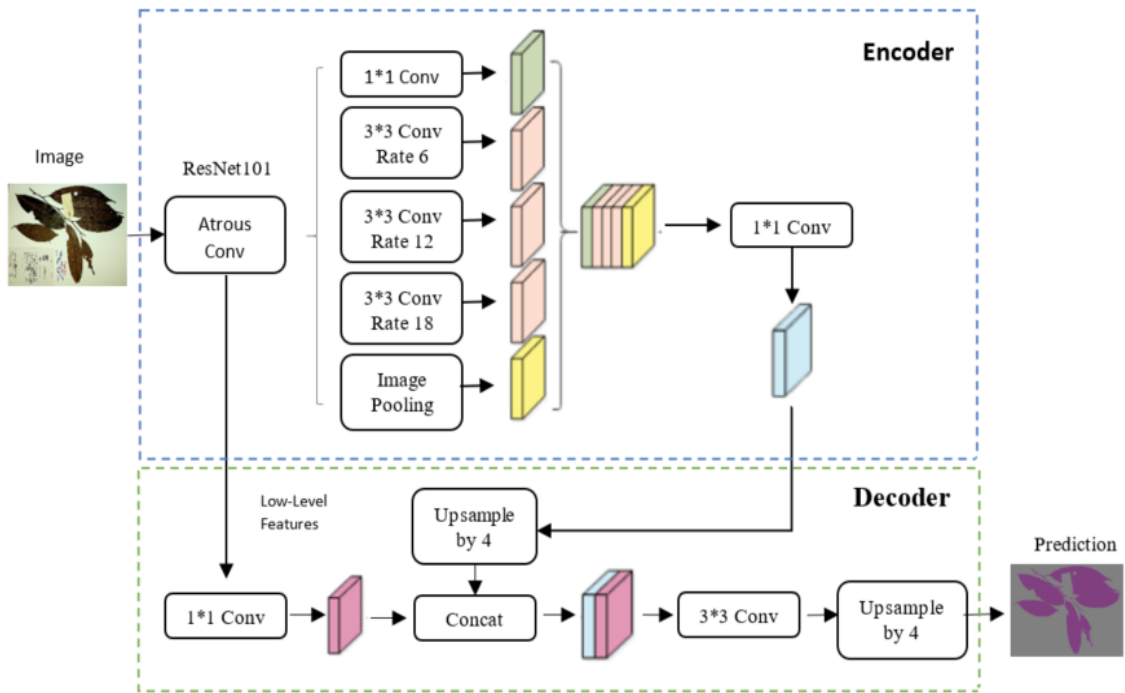
\includegraphics[width=0.9\textwidth]{chapters/chapter1/images/Figure22.png}
    \caption{DeepLabv3+ architecture \parencite{hussein2020semantic}.}
    \label{fig:DeepLabv3+}
\end{figure}

% \section{Challenges of Deep Learning in Agricultural Contexts}

% Despite the promising performance of deep learning and object detection in various fields, their application in agriculture presents a range of specific challenges. One of the primary issues is the limited availability of large, annotated agricultural datasets, which hampers the training of robust and generalizable models. Unlike natural image datasets like ImageNet, agricultural datasets often suffer from class imbalance, incomplete labeling, and domain specificity (e.g., crop types, diseases, and environmental conditions) \parencite{alzubaidi2021review}.

% Another challenge is the high intra-class variability and low inter-class variability found in agricultural images. For instance, symptoms of different diseases may look visually similar, or the same disease may appear differently across plant species and growth stages. Additionally, variations in lighting, occlusion by leaves, overlapping plants, and background clutter significantly affect detection performance \parencite{alzubaidi2021review}.

% The seasonal and geographic diversity further complicates the generalization of models trained on limited datasets. Moreover, the deployment of deep learning models in real agricultural environments must consider limited computing resources, especially for edge or mobile devices used in fields.

% Lastly, ensuring the interpretability and trustworthiness of AI decisions is crucial in agricultural contexts, as these technologies directly impact yield, resource use, and farmers’ livelihoods. Addressing these challenges requires collaborative efforts in data collection, annotation, model adaptation, and efficient deployment strategies \parencite{alzubaidi2021review}.

\section{Conclusion}
In this chapter, we explored key deep learning concepts and models used for image-based recognition tasks, focusing on classification, object detection, and semantic segmentation. These techniques are essential for automating and improving agricultural workflows, especially in crop health monitoring. Building on this foundation, the next chapter will introduce remote sensing technologies and investigate how their integration with deep learning and machine learning can enable the accurate and scalable early detection of wheat diseases. 
\chapter{Threats to Wheat Production: Disease Identification and the Shift Toward Smart Agriculture}

\section{Introduction}

Wheat is a crucial global crop, but its production is threatened by various diseases and insect pests, leading to significant yield losses. Traditional detection and control methods are often ineffective, highlighting the need for improved solutions. 

This chapter explores common wheat diseases and pests, their impact on agriculture, and the importance of timely detection. It also discusses strategies for enhancing disease control and the challenges of implementing smart agricultural technologies.



\section{Motivation for the Protection of Wheat Crops}

Wheat is an ancient and vital food crop that provides energy and feeds billions of people around the world (see Figure~\ref{fig:Figure01}). Its demand is growing quickly because it’s used in many affordable food products and plays a big role in global food security. The FAO (Food and Agriculture Organization) estimates that by 2050, the world will need about 840 million tonnes of wheat, up from 642 million tonnes today \parencite{sharma2015wheat}. This doesn’t even include the extra needs like animal feed or the impact of climate change.

To meet this growing demand, developing countries need to increase wheat production by 77\%, mostly by improving how much wheat is grown on the same land \parencite{sharma2015wheat}. But this is becoming harder, as wheat productivity is slowing down and diseases are becoming a bigger problem. If we don’t manage pests and diseases properly, wheat production could fall short of what the world needs.

That’s why it's important to invest in research, use better farming methods, and grow disease-resistant wheat. Protecting this essential crop is key to making sure we have enough food for the future.


\begin{figure}[H]
    \centering
    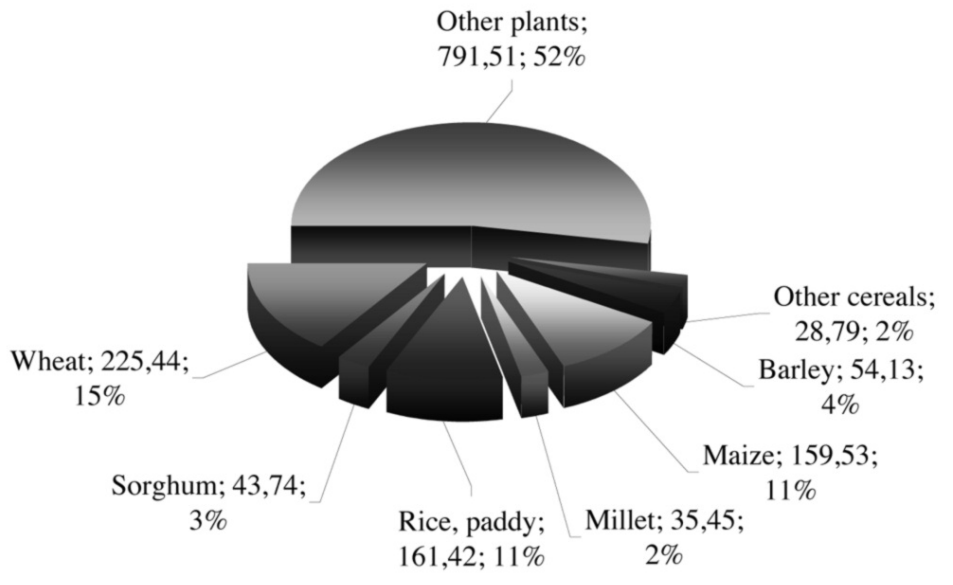
\includegraphics[width=0.7\textwidth]{chapters/chapter2/images/Figure01.png}
    \caption{Division of sowing area in the world in 2009 (in million hectares and percentage) Source: FAO, 2011}
    \label{fig:Figure01}
\end{figure}

\section{Wheat growth stages}
Wheat growth follows a series of distinct developmental stages (Figure~\ref{fig:WheatStages}), each with specific environmental needs and a direct impact on crop health and yield \parencite{shafi2020multi}. The key stages are:

\begin{itemize}
    \item \textbf{Seeding:} The initial stage where seeds germinate and seedlings emerge. Adequate soil moisture and suitable temperatures are essential for successful crop establishment.
    
    \item \textbf{Tillering:} The plant produces side shoots (tillers), which increase potential yield. This stage depends on sufficient nutrients and water.
    
    \item \textbf{Booting:} The wheat head develops inside the leaf sheath. Stress at this stage can reduce the number of spikelets and affect grain development.
    
    \item \textbf{Heading:} The spike emerges and flowering occurs. This is a sensitive period where drought or heat can severely impact pollination and grain set.
    
    \item \textbf{Ripening:} Grains mature and the plant loses its green color. Proper conditions are needed for effective grain filling and harvest readiness.
\end{itemize}

\begin{figure}[H]
    \centering
    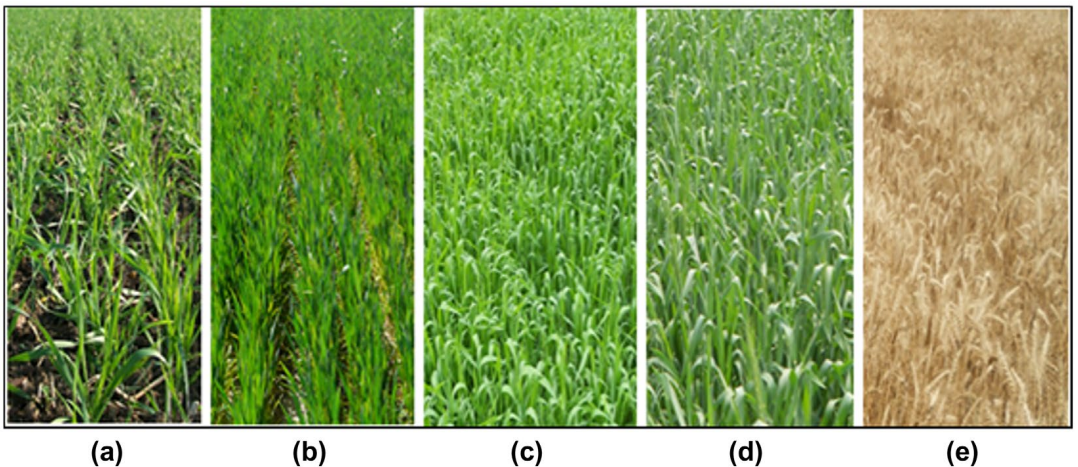
\includegraphics[width=0.7\textwidth]{chapters/chapter2/images/WheatStages.png}
    \caption{ wheat crop growth stages: (a) Tillering; (b) Jointing; (c) Booting; (d) Heading; and (e) Ripening \parencite{kumar2018estimation}}
    \label{fig:WheatStages}
\end{figure}



\section{Wheat Diseases: Types and Impacts}

Wheat diseases are influenced by several factors, including plant resistance, spore density, temperature, and environmental conditions, especially the presence of moisture on plant surfaces, which facilitates infection. While some fungi are host-specific, others can infect a wide range of plants. Symptoms can differ greatly, making accurate identification essential. Researchers primarily rely on fungal morphology for diagnosis. A clear understanding of these diseases is key to effective management and control. The following classification (Figure ~\ref{fig:Figure02}) outlines the major wheat diseases, grouped by their causes and the plant parts they affect.

\begin{figure}[H]
    \centering
    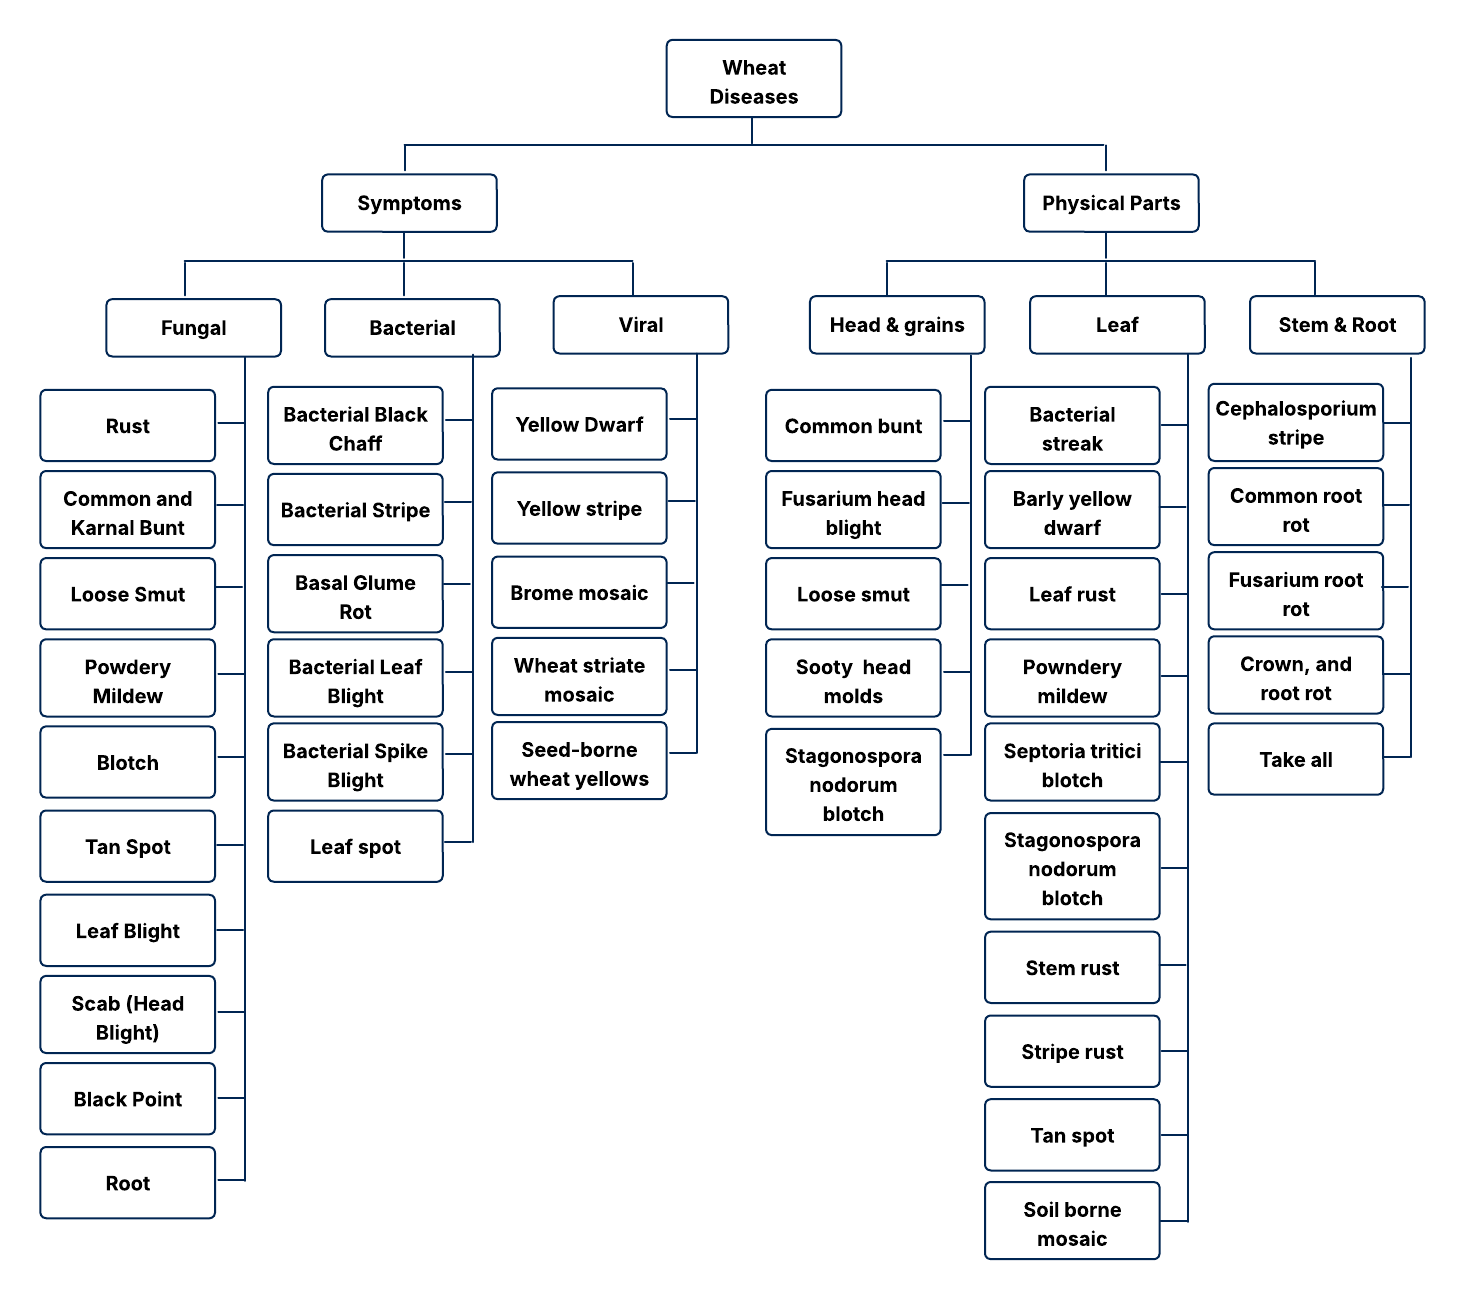
\includegraphics[width=0.9
    \textwidth]{chapters/chapter2/images/Figure02.png}
    \caption{Taxonomy of wheat diseases \protect\parencite{haider2021wheat}}
    \label{fig:Figure02}
\end{figure}

\subsection{Leaf Rust (Brown Rust)} 

\begin{figure}[H]
    \centering
    \begin{minipage}{0.65\textwidth}
        
        Leaf rust, caused by \textit{Puccinia triticina}, appears as small, circular, orange to brown pustules on the upper surfaces of leaves and leaf sheaths. It spreads through wind-borne spores and develops quickly in moist conditions at around 20°C. New spores form every 10–14 days if conditions are favorable. As plants mature or conditions worsen, black spores may appear (as shown in Figure~\ref{fig:Figure03}). 
        
        This disease affects wheat, triticale, and related grasses and is common in temperate cereal-growing regions. Severe infections reduce grain yield, kernel number, weight, and quality \parencite{duveiller2012wheat}.
    \end{minipage}%
    \hfill
    \begin{minipage}{0.3\textwidth}
        \centering
        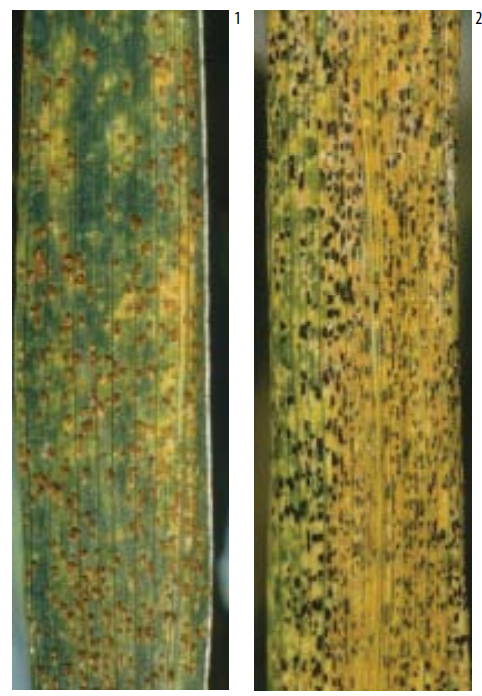
\includegraphics[width=0.6\linewidth]{chapters/chapter2/images/Figure03.png}
        
        \captionof{figure}{Leaf rust with Brown spores (1), Leaf rust with Black spores (2) \protect\parencite{duveiller2012wheat}}
        \label{fig:Figure03}
    \end{minipage}
\end{figure}




\subsection{Stem Rust (Black Rust)}

\begin{figure}[H]
    \centering
    \begin{minipage}{0.65\textwidth}
        
        Stem rust, caused by \textit{Puccinia graminis}, appears as dark reddish-brown pustules on leaves, stems, and spikes (as observed in Figure~\ref{fig:Figure04}). Light infections show scattered pustules, while severe cases cause them to merge. Before pustules form, small flecks may appear, and infected areas feel rough. The disease spreads through wind-borne spores and develops quickly in moist conditions with temperatures around 20°C. New spores can form in 10–15 days. It affects wheat, barley, triticale, and related grasses and is common in temperate cereal regions. Severe infections can reduce grain weight and quality and, in extreme cases, lead to total crop loss \parencite{duveiller2012wheat}.
    \end{minipage}%
    \hfill
    \begin{minipage}{0.3\textwidth}
        \centering
        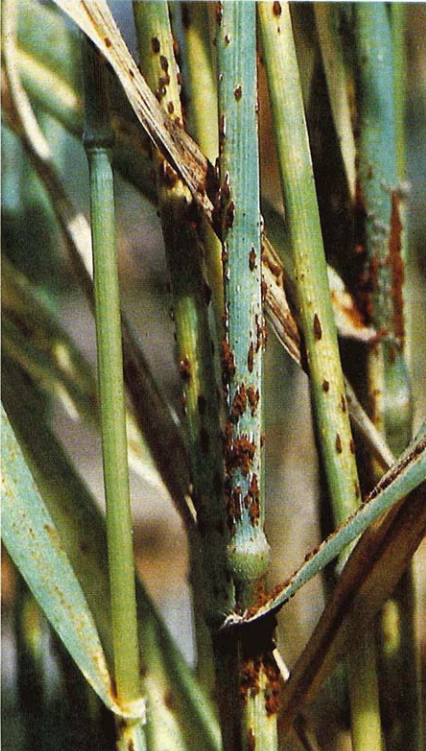
\includegraphics[width=0.6\linewidth]{chapters/chapter2/images/Figure04.png}
        \captionof{figure}{Stem rust \protect\parencite{duveiller2012wheat}}
        \label{fig:Figure04}
    \end{minipage}
\end{figure}


\subsection{Stripe Rust (Yellow Rust)}
\begin{figure}[H]
    \centering
    \begin{minipage}{0.65\textwidth}
        
        Stripe rust, caused by \textit{Puccinia striiformis}, appears as yellow to orange-yellow pustules forming narrow stripes on leaves, leaf sheaths, necks, and glumes (as seen in Figure~\ref{fig:Figure05}). It spreads through wind-borne spores and develops quickly in moist conditions at temperatures between 10–20°C but slows down above 25°C. Severe infections reduce grain yield, kernel number, weight, and quality \parencite{duveiller2012wheat}.
    \end{minipage}%
    \hfill
    \begin{minipage}{0.3\textwidth}
        \centering
        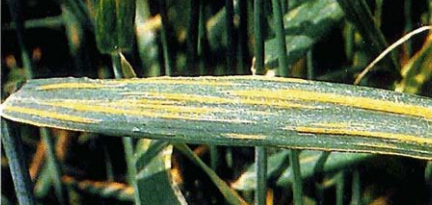
\includegraphics[width=0.9\linewidth, angle=90]{chapters/chapter2/images/Figure05.png}
        \captionof{figure}{Stripe rust \protect\parencite{duveiller2012wheat}}
        \label{fig:Figure05}
    \end{minipage}
\end{figure}

\subsection{Blotch Diseases} 

\begin{figure}[H]
    \centering
    \begin{minipage}{0.55\textwidth}
        
        The blotch diseases, which include Septoria tritici blotch (STB), Septoria nodorum blotch (SNB), and tan spot (TS) (as presented in Figure~\ref{fig:Figure06}), are caused by the  \textit{Ascomycete fungi Zymoseptoria tritici}, \textit{Parastagonospora nodorum}, and \textit{Pyrenophora tritici-repentis}, respectively \parencite{figueroa2018review}.
    \end{minipage}%
    \hfill
    \begin{minipage}{0.4\textwidth}
        \centering
        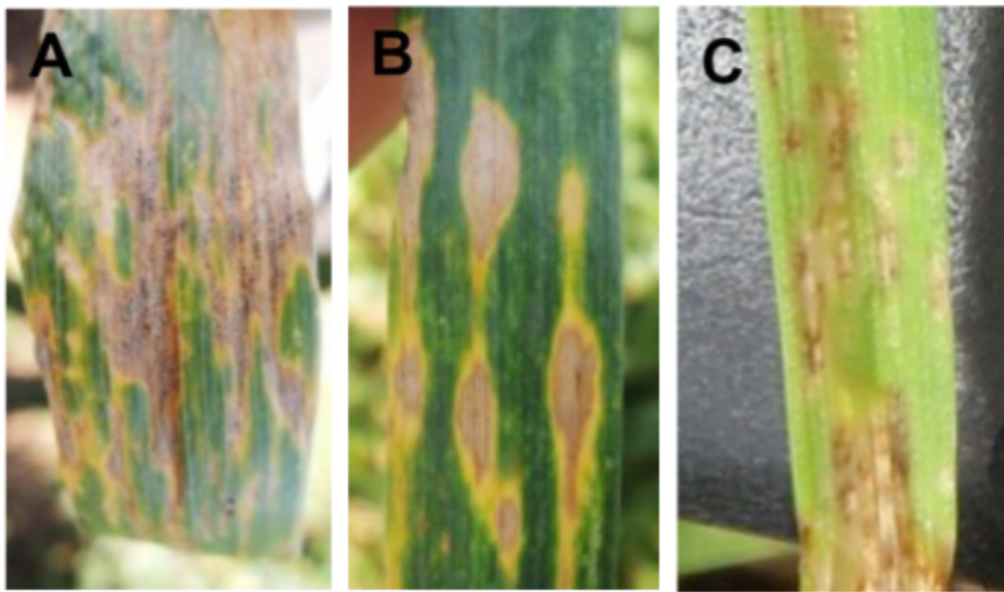
\includegraphics[width=0.9\linewidth]{chapters/chapter2/images/Figure06.png}
        \captionof{figure}{Symptoms of foliar blotch diseases. (A) Septoria tritici blotch. (B) Tan spot. (C) Septoria nodorum blotch \protect\parencite{figueroa2018review}}
        \label{fig:Figure06}
    \end{minipage}
\end{figure}

\subsection{Fusarium Head Blight (FHB)}

\begin{figure}[H]
    \centering
    \begin{minipage}{0.55\textwidth}
        
        Fusarium head blight (FHB), also known as wheat scab or ear blight, is a major disease of wheat caused primarily by the Ascomycete fungus \textit{Fusarium graminearum} (Fg). It can also be caused by other regional \textit{Fusarium} species \parencite{figueroa2018review}.\\
        Fusarium head blight appears as dark, oily florets with pinkish spores (as seen in Figure~\ref{fig:Figure07}). Infected kernels may be covered in white fungal growth. The disease spreads in warm, humid conditions (10–28°C), infecting spikes during flowering and spreading between florets. It affects all small grain cereals and is found in most soils and crop residues. Severe infections can reduce yields by over 50\% and lower grain quality. Contaminated grain may contain harmful mycotoxins, making it unsafe for humans and animals \parencite{duveiller2012wheat}.
    \end{minipage}%
    \hfill
    \begin{minipage}{0.4\textwidth}
        \centering
        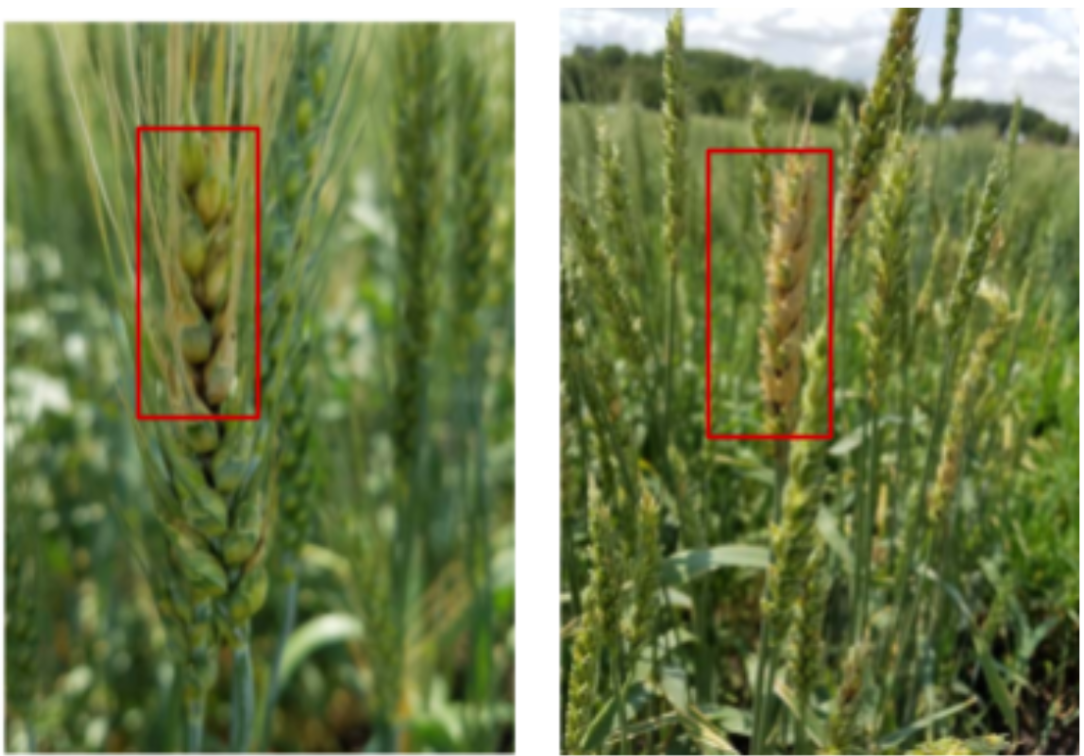
\includegraphics[width=0.95\linewidth]{chapters/chapter2/images/Figure07.png}
        \captionof{figure}{Symptoms of Fusarium head blight/scab: The left image shows early infection signs manifested as a partially bleached wheat head, while the right image illustrates advanced infection of \textit{Fusarium graminearum} \protect\parencite{figueroa2018review}.}
        \label{fig:Figure07}
    \end{minipage}
\end{figure}



\subsection{Loose Smut}

\begin{figure}[H]
    \centering
    \begin{minipage}{0.65\textwidth}
        
        Loose smut, caused by \textit{Ustilago tritici}, replaces wheat spikes with black fungal spores (as observed in Figure~\ref{fig:Figure08}), which are later dispersed by wind. The fungus infects wheat flowers and stays dormant in kernels until germination. It then grows with the plant, destroying floral parts at flowering. The disease thrives in cool, humid conditions and is found wherever wheat is grown. Yield losses depend on infection levels, usually below 1\% but sometimes reaching 30\% \parencite{duveiller2012wheat}.
    \end{minipage}%
    \hfill
    \begin{minipage}{0.3\textwidth}
        \centering
        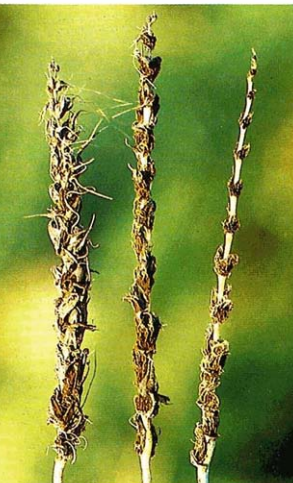
\includegraphics[width=0.9\linewidth]{chapters/chapter2/images/Figure08.png}
        \captionof{figure}{Loose smut \protect\parencite{duveiller2012wheat}}
        \label{fig:Figure08}
    \end{minipage}
\end{figure}


\subsection{Powdery mildew} 

\begin{figure}[H]
    \centering
    \begin{minipage}{0.55\textwidth}
        
        Powdery mildew (Figure~\ref{fig:Figure09}), caused by \textit{Blumeria graminis f. sp. tritici}, affects wheat globally, particularly in cool, dry climates, and can cause yield losses ranging from 10\% to 40\%, with severe cases leading to seedling or tiller death \parencite{singh2023wheat}.
    \end{minipage}%
    \hfill
    \begin{minipage}{0.4\textwidth}
        \centering
        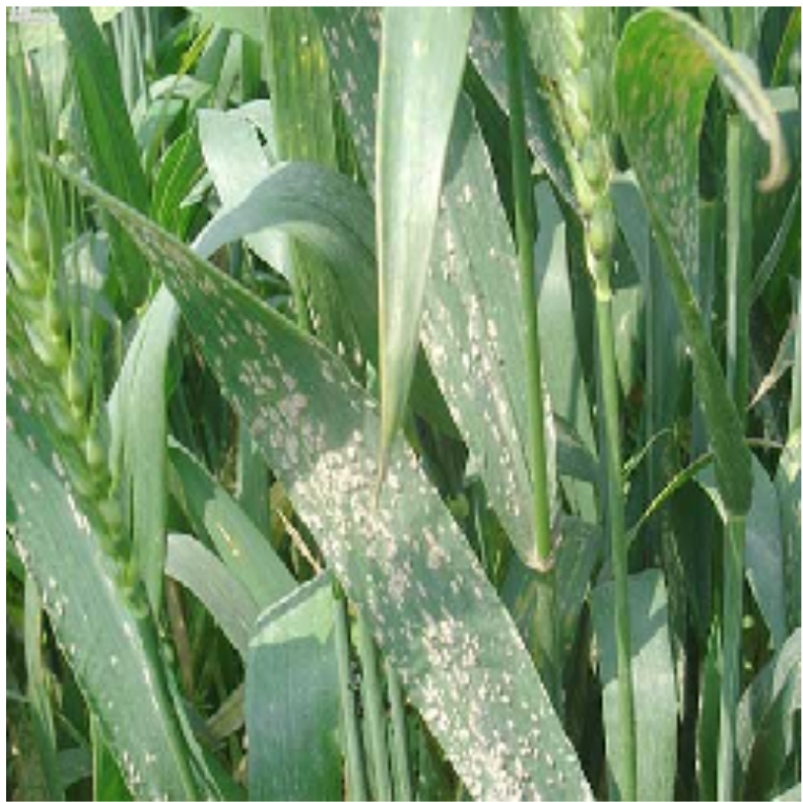
\includegraphics[width=0.5\linewidth]{chapters/chapter2/images/Figure09.png}
        \captionof{figure}{Powdery mildew from Kaggle dataset ‘Wheat Plant Diseases.'}
        \label{fig:Figure09}
    \end{minipage}
\end{figure}

\subsection{Common Root Rot}

\begin{figure}[H]
    \centering
    \begin{minipage}{0.65\textwidth}
        
        Common root rot, caused by \textit{Cochliobolus sativus}, \textit{Fusarium spp}, and \textit{Pythium spp}, darkens and weakens wheat roots, crowns, and stems (as illustrated by Figure~\ref{fig:Figure10}), sometimes leading to plant lodging and white spikes before maturity. Early infections can cause seedling death.
        The disease spreads from infected crop debris, thriving in different soil conditions: \textit{C. sativus} in warm, dry soils and \textit{Fusarium} and \textit{Pythium} in cool, moist soils. Found in temperate regions, it rarely causes major outbreaks but can lead to localized losses due to reduced plant growth and yield \parencite{duveiller2012wheat}.
    \end{minipage}%
    \hfill
    \begin{minipage}{0.3\textwidth}
        \centering
        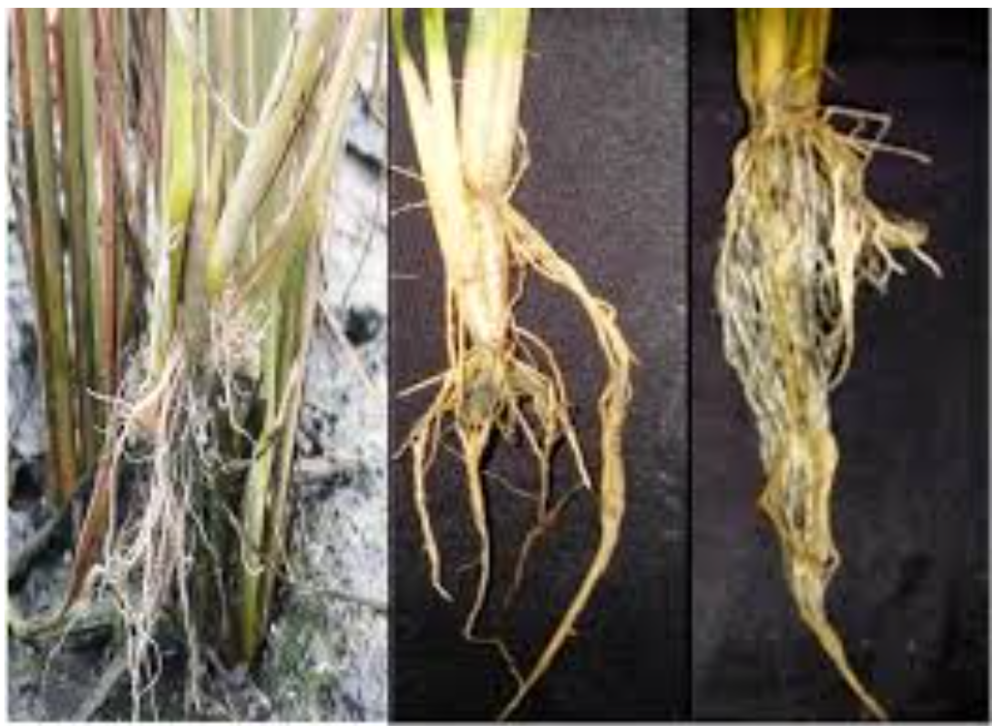
\includegraphics[width=0.8\linewidth]{chapters/chapter2/images/Figure10.png}
        \captionof{figure}{Common root rot from Kaggle dataset ‘Wheat Plant Diseases.’}
        \label{fig:Figure10}
    \end{minipage}
\end{figure}


\section{Common Insect Pests in Wheat Cultivation}
Wheat is affected by several insect pests that can seriously reduce yield and quality. Below are some of the most common pests and their impacts (see \autoref{fig:wheat-pests}).
\begin{itemize}
    \item \textbf{Aphids:} Aphids are soft-bodied, transparent insects that feed on wheat leaves and grain heads, causing yellowing, leaf rolling, and poor pollination, especially during early growth. Their sap-sucking damages crops, and the honeydew they excrete promotes black sooty mold, reducing photosynthesis and leading to yield losses of 20–80\% \parencite{duveiller2012wheat,farook2019insect}.

    \item \textbf{Cereal leaf beetle:} Adult cereal leaf beetles are 4–5 mm long with a black head, light brown thorax, and shiny blue-green wings. Larvae are initially yellow but turn into a black mass due to accumulated fecal material. The main symptom of infestation is distinct longitudinal stripes on leaves caused by the feeding of both adults and larvae. Infestations can lead to yield losses of 14\% to over 25\% in winter and fall-sown spring wheat \parencite{duveiller2012wheat}.

    \item \textbf{Armyworm:} The armyworm (Mythimna separata) is a wheat pest. Adult moths are stout and pale brown, while larvae have orange, white, and brown stripes, along with black spots on their prolegs. Caterpillars cause significant damage by swarming from field to field, feeding on seedling leaves and ear heads, which halts plant growth \parencite{farook2019insect}.

    \item \textbf{Brown wheat mite:} The brown wheat mite, found in rainfed wheat areas, has only females that lay red eggs in winter and white-covered eggs in summer. They damage crops by sucking sap, causing silvery flecks, yellowing leaves, and reduced grain quality. Mites are active in daylight and do not form webs. Infestations start in December–January and last until maturity, with winter rains limiting their spread \parencite{kashyap2018identification}.

    \item \textbf{Pink stem borer:} The pink stem borer (Sesamia inferens) is an oriental pest that originally affected rice but has adapted to wheat in North-Western India. Its larvae feed inside wheat stems, causing "dead hearts" and "white heads," leading to yield losses over 11\%. Damage symptoms in wheat are similar to those in rice \parencite{farook2019insect}.

    \item \textbf{Sawfly:} Sawflies produce one generation per year, with larvae overwintering in straw. The legless white larvae bore into wheat stems, weakening plants, causing poor head development, and making them prone to lodging. While infestations are patchy, the wheat stem sawfly (Cephus cinctus) can cause severe localized yield losses \parencite{duveiller2012wheat}.

    \item \textbf{Slugs, Snails, Grasshoppers, and Crickets:} These are widespread pests affecting wheat and other plants. They damage crops by chewing leaves, causing a frayed appearance in mature plants. While their presence is often localized, large infestations can significantly impact plant health and yield worldwide.

    \item \textbf{Wireworm:} Wireworms are yellow to brown larvae with six short legs that feed on wheat kernels, consuming the endosperm and leaving only the seed coat. They attack young seedlings, causing "damping off" symptoms and damaging crops early on. Their presence can significantly affect wheat growth and yield, making timely identification and control crucial \parencite{farook2019insect}.
\end{itemize}

\begin{figure}[H]
    \centering
    \subfloat[Aphids \protect\parencite{farook2019insect}]{
        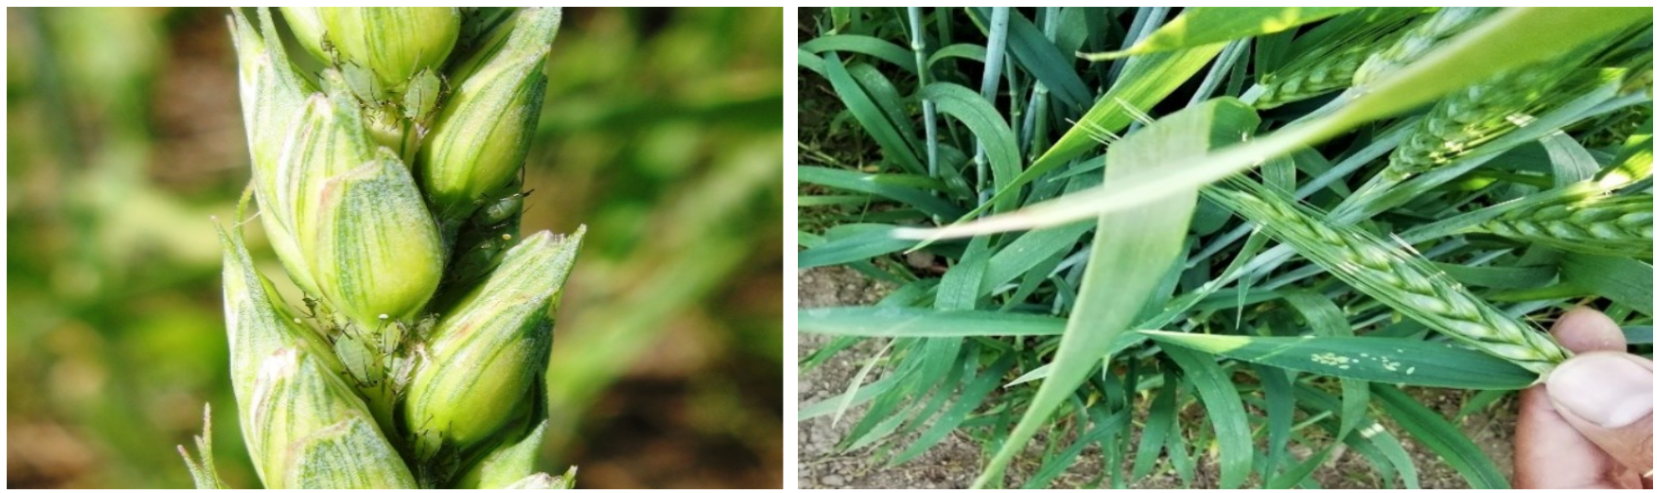
\includegraphics[width=0.3\textwidth,height=0.17\textwidth]{chapters/chapter2/images/Figure11.png}
    }
    \subfloat[Cereal leaf beetle \protect\parencite{farook2019insect}]{
        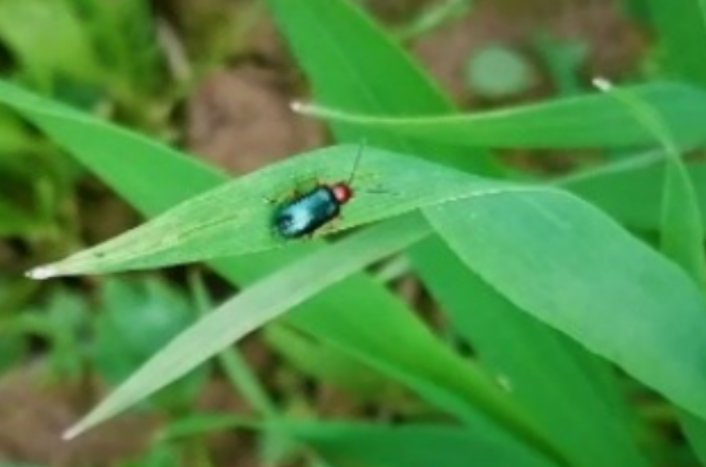
\includegraphics[width=0.3\textwidth,height=0.17\textwidth]{chapters/chapter2/images/Figure12.png}
    }
    \subfloat[Armyworm \protect\parencite{farook2019insect}]{
        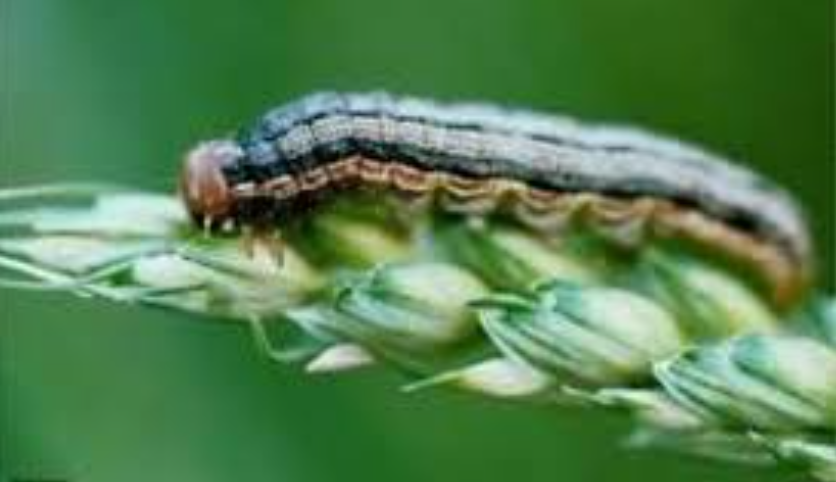
\includegraphics[width=0.3\textwidth,height=0.17\textwidth]{chapters/chapter2/images/Figure13.png}
    }\\[-0.2em]

    \subfloat[Brown wheat mite \protect\parencite{kashyap2018identification}]{
        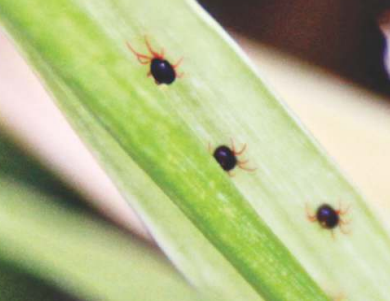
\includegraphics[width=0.3\textwidth,height=0.17\textwidth]{chapters/chapter2/images/Figure15.png}
    }
    \subfloat[Pink stem borer \protect\parencite{farook2019insect}]{
        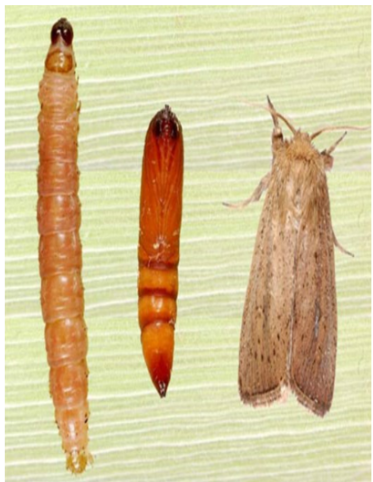
\includegraphics[width=0.3\textwidth,height=0.17\textwidth]{chapters/chapter2/images/Figure16.png}
    }
    \subfloat[Sawfly (Kaggle)]{
        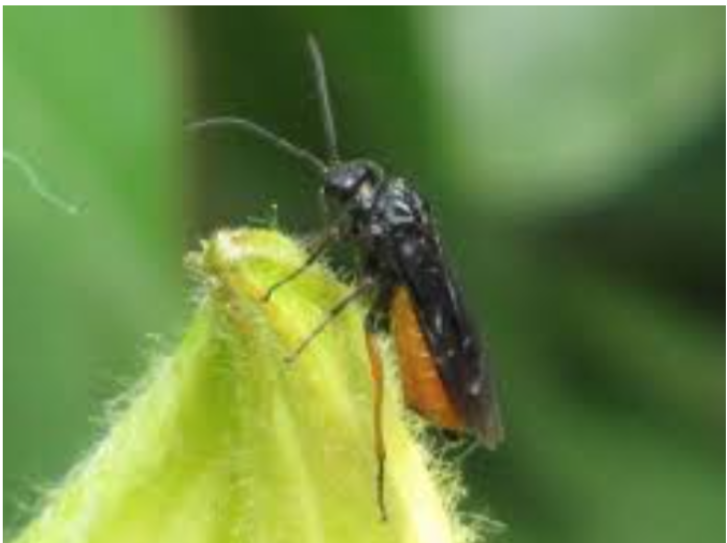
\includegraphics[width=0.3\textwidth,height=0.17\textwidth]{chapters/chapter2/images/Figure17.png}
    }\\[-0.2em]

    \subfloat[Grasshoppers (Kaggle)]{
        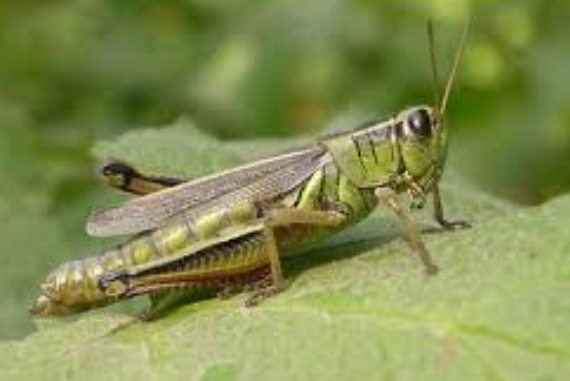
\includegraphics[width=0.3\textwidth,height=0.17\textwidth]{chapters/chapter2/images/Figure18.png}
    }
    \subfloat[Wireworm \protect\parencite{farook2019insect}]{
        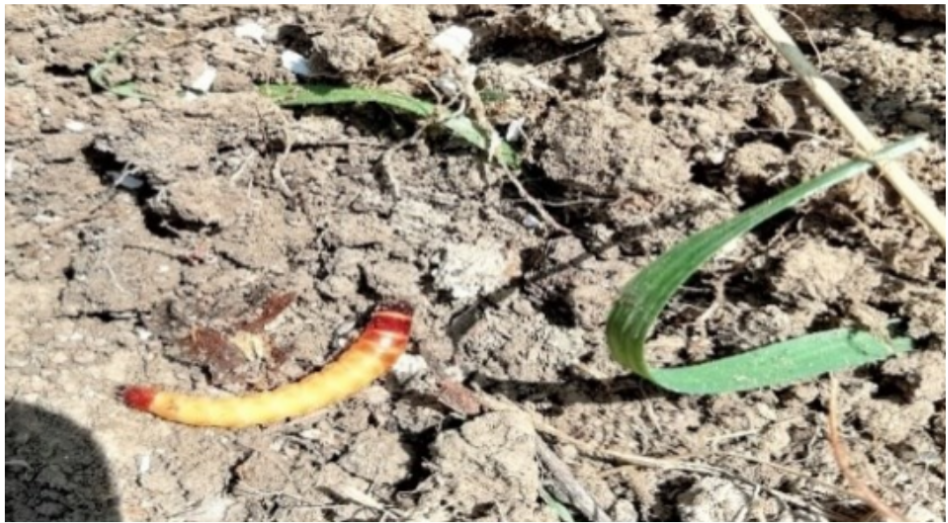
\includegraphics[width=0.3\textwidth,height=0.17\textwidth]{chapters/chapter2/images/Figure19.png}
    }

    \caption{Common pests affecting wheat crops.}
    \label{fig:wheat-pests}
\end{figure}


\section{Enhancing Wheat Disease Control Strategies}

Effective wheat disease management combines traditional farming practices with modern technologies. Together, they offer a balanced approach to reducing disease impact and improving crop health.

\subsection{Usual Instruments (Classic Methods)}
These are long-standing approaches that provide the foundation for managing wheat diseases \parencite{mehta2014wheat}. The following practices have been widely used to reduce disease pressure and support healthy crop development.

\begin{itemize}
    \item \textbf{Crop Rotation:} Rotating wheat with non-host crops reduces the buildup of soil-borne pathogens and interrupts disease cycles.
    \item \textbf{Tillage:} Tillage affects disease development by influencing residue decomposition and soil pathogen levels; conservation tillage can increase some necrotrophic diseases.
    \item \textbf{Healthy Seeds:} Clean, pathogen-free seeds minimize seed-borne disease transmission and ensure strong early crop establishment.
    \item \textbf{Soil Management:} Managing soil pH, structure, and nutrient balance helps prevent stress-related susceptibility and supports healthier root systems.
    \item \textbf{Fertilizer Use:} Balanced fertilization strengthens plant defense mechanisms, while over- or under-fertilization can predispose plants to infection.
    \item \textbf{Diversification of Cultivars and Sowing Dates:} Altering cultivars and planting schedules helps reduce the uniformity that pathogens exploit and spreads risk across environments.
    \item \textbf{Use of Resistant Cultivars:} Cultivars bred for specific, partial, or generalized resistance can significantly reduce disease severity, especially when tailored to local pathogen races.
    \item \textbf{Alternative Eco-Friendly Practices:} Methods like field sanitation, residue management, and proper spacing contribute to reducing pathogen survival and disease spread.
\end{itemize}

\subsection{Technological Tools}
Complementing traditional methods, the following tools, rooted in smart agriculture, offer modern solutions to enhance the effectiveness and precision of wheat disease management.

\begin{itemize}
    \item \textbf{Remote Sensing:} Remote sensing using unmanned aerial vehicle-mounted multispectral sensors enables high-resolution monitoring of wheat canopy characteristics across different growth stages. By analyzing spectral bands (Green, Red, Red Edge, Near Infrared), the system captures critical indicators of plant health, canopy structure, and stress conditions, supporting precise and timely crop management \parencite{zhang2025precision}.
    \item \textbf{Disease Forecast Modeling:} Weather-based and biological models are used to predict disease outbreaks and support timely interventions \parencite{mehta2014wheat}.
    \item \textbf{Computer Vision:} Enables automated analysis of crop images for monitoring wheat growth, detecting diseases, and assessing yield. It plays a crucial role in real-time decision-making by processing visual data from the field \parencite{ghazal2024computer}.
    \item \textbf{AI and Machine Learning Algorithms:} Used to interpret complex image data, these algorithms support tasks like disease classification, crop health prediction, and optimizing farm operations by learning from patterns in large agricultural datasets \parencite{ghazal2024computer}.
    \item \textbf{Autonomous Robotic Platforms and Drones:} Facilitate efficient field data collection, spraying, and crop monitoring. These tools reduce manual labor and enable precise, targeted interventions across large wheat fields \parencite{ghazal2024computer}.
    \item \textbf{Precision Agriculture Systems:} Precision agriculture systems integrate technologies like the Global Positioning System (GPS) and the Internet of Things  (IOT) to manage field variability. These technologies help optimize the use of inputs (e.g., water, fertilizer) and support sustainable, data-driven wheat farming \parencite{ghazal2024computer}.
\end{itemize}

% \section{Challenges Facing the Integration of Smart Agricultural Systems}
% Fully automated smart farming faces both technical and practical challenges. A major obstacle is the generalization of computer vision models across diverse field conditions like lighting, weather, soil, and crop types, which complicates real-time deployment. Robust decision-making in unpredictable outdoor environments also remains difficult, and integrating the full pipeline from image capture to treatment is still under development \parencite{ghazal2024computer}.

% On the technical side, communication protocols often support only short distances, limiting scalability. Many devices rely on batteries, reducing operational time. Additionally, processing the large volumes of data generated introduces computational bottlenecks, alongside concerns about privacy, trust, and security in data handling \parencite{idoje2021survey}.



\section{Conclusion}

The increasing threat of wheat diseases and insect pests necessitates more effective and timely detection solutions. While conventional and technological tools provide some control, integrating advanced technologies such as Machine Learning, Deep Learning, and Remote Sensing presents a more promising direction. These intelligent systems enable early detection and precise monitoring, paving the way for smarter agricultural practices. The following chapter explores Deep Learning in greater detail and its role in transforming wheat disease detection.

\chapter{Literature Review}

\section{Introduction}
Over the past decade, machine learning and deep learning have shown great potential in addressing challenges in early disease detection and pest identification in agriculture. This literature review critically examines current wheat disease classification and pest detection research using deep learning techniques. It explores the evolution from traditional methods to modern AI-driven approaches, highlighting the strengths and limitations of each. Key challenges such as limited data availability, model complexity, and interpretability are discussed in the context of real-world applications. The review also identifies major trends and research gaps in the field. By synthesizing these findings, it aims to provide insights into the future of smart agriculture. This chapter lays the groundwork for the thesis’s proposed deep learning-based system. The goal is to enhance disease and pest management in wheat crops. Ultimately, it aims to contribute to more efficient, sustainable farming practices.

\section{Approaches in Data Collection and Preprocessing }
This section discusses various methods employed in the literature for gathering data, handling challenges such as low-quality or irrelevant images, and preprocessing techniques that prepare datasets for effective utilization in classification and detection tasks.

\subsection{Data Collection}
The initial and foundational step in developing deep learning models for wheat disease classification is the acquisition of high-quality and diverse image data. This data can be sourced through various means, including manual and automated methods. Common sources include drone-mounted or mobile device cameras, which allow for the real-time capture of wheat leaf images under natural field conditions. Public datasets also play a crucial role; for instance, the "Wheat Leaf Dataset" available on Kaggle, utilized by \parencite{ramadan2024improving}, and the "Wheat Disease Detection" dataset, employed by \parencite{reis2024integrated}, offer extensive repositories of labeled images. In addition to these, hybrid data collection strategies are often employed. \parencite{hassan2024wheat}, for example, combined images obtained from field visits, Kaggle datasets, and internet sources to enrich their training data. This diversity in data sources helps improve the robustness and generalization capability of the resulting models.


\subsection{Data Preprocessing}
Data preprocessing plays a crucial role in improving the quality and relevance of input images for deep learning models. This process typically begins with the elimination of low-quality images where disease symptoms are poorly visible \parencite{yao2024yolo} and the cropping of extraneous image regions to concentrate on areas of diagnostic interest. To further enhance the visual quality, advanced contrast enhancement techniques such as Contrast Limited Adaptive Histogram Equalization (CLAHE), contrast stretching, and the hypercolumn technique (Figure~\ref{fig:CLAHE}) are commonly employed to improve image contrast and brightness, as discussed by \parencite{reis2024integrated} and \parencite{fang2023lightweight}. These methods significantly improve image contrast and brightness, making subtle disease features more discernible and thereby facilitating more accurate classification. Additionally, to isolate the region of interest and reduce background noise, methods such as background removal, color thresholding, and edge detection are utilized \parencite{alharbi2023wheat}, ensuring that only the most relevant image features are presented to the model.


\begin{figure}[H] % 'H' needs \usepackage{float}
    \centering
    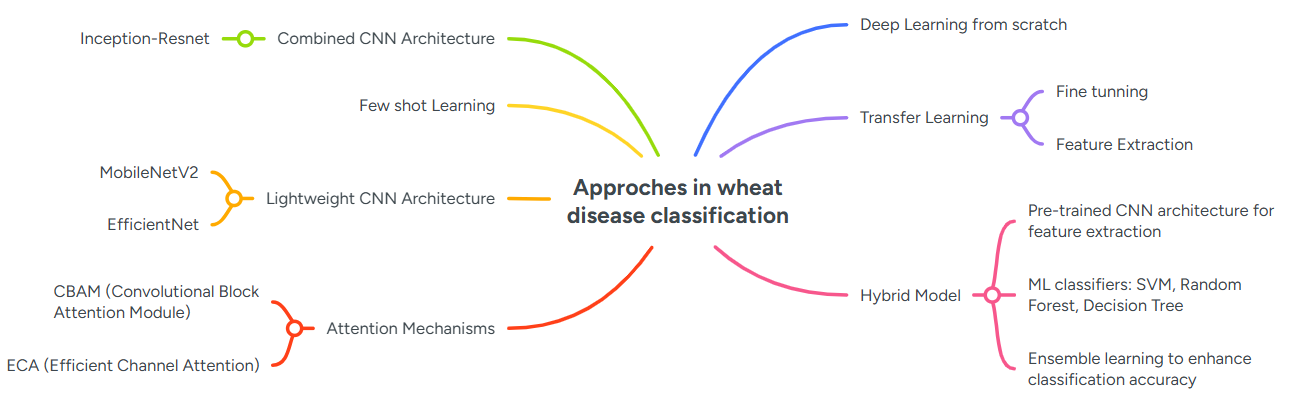
\includegraphics[width=0.8\textwidth]{chapters/chapter3/images/Figure01.png}
    \caption{Sub-data samples of the wheat disease original dataset obtained by the CLAHE, Contrast stretching, and hypercolumn technique \parencite{reis2024integrated}.}
    \label{fig:CLAHE}
\end{figure}

\subsection{Data augmentation}

Data augmentation is extensively employed to mitigate class imbalance and enhance dataset diversity, thereby improving the generalization capabilities of deep learning models. Common augmentation techniques include random rotations, cropping, zooming, flipping, and contrast adjustments (Figure~\ref{fig:Dataaugmentation}), which artificially expand the training dataset by introducing varied visual representations of the original images \parencite{nagpal2024hybrid,hassan2024wheat,nigam2023deep}.

\begin{figure}[H] % 'H' needs \usepackage{float}
    \centering
    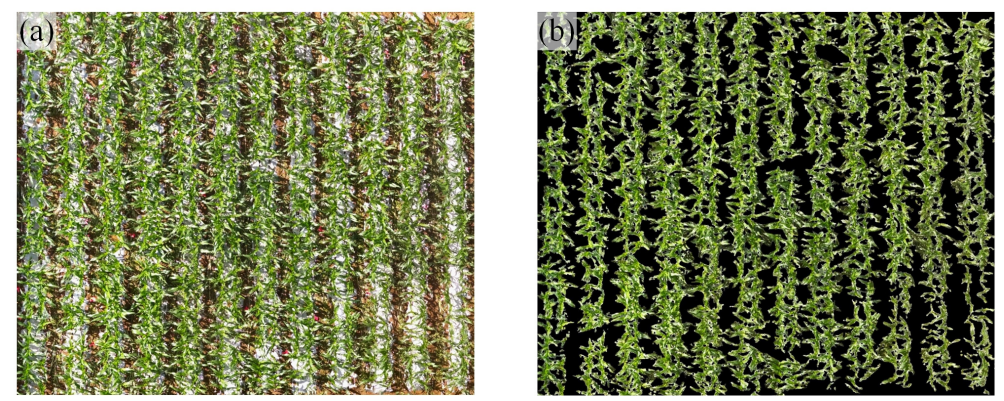
\includegraphics[width=0.6\textwidth]{chapters/chapter3/images/Figure02.png}
    \caption{Data augmentation techniques \parencite{nagpal2024hybrid}.}
    \label{fig:Dataaugmentation}
\end{figure}

\parencite{ramadan2024improving} use four augmentation techniques enhance dataset diversity and address class imbalance: CycleGAN, which generates realistic synthetic images through unpaired image-to-image translation; ADASYN, which adaptively oversamples difficult minority class instances; SMOTE, which creates synthetic samples by interpolating between minority class neighbors; and SMOTE-Tomek, a hybrid method that combines SMOTE with Tomek links to both oversample and remove noisy boundary samples.




\section{Approaches in Wheat Disease Classification}

Various classification models have been employed in the literature to address wheat disease classification effectively. These approaches, preprocessing techniques, datasets, classification categories, and results are summarized in Table~\ref{tab:Table 01}, which provides a comparative overview of the most recent and relevant studies in this domain.

\textbf{Transfer Learning Approaches:} \parencite{jiang2022evaluation} compares three CNN training strategies for wheat disease identification (Figure~\ref{fig:TrainingStrategies}): training from scratch, fixed feature extraction, and transfer learning with fine-tuning.

\begin{itemize}
  \item \textbf{Training from scratch:} The entire CNN is trained from the beginning with randomly initialized weights using only the target dataset (FWDI). This approach allows full customization but requires a large amount of data and significant computational power.

  \item \textbf{Fixed feature extraction:} In this strategy, a pre-trained CNN is employed as a fixed feature extractor, where all convolutional layers are frozen to preserve the learned representations, and only the final classification layers—such as the fully connected, batch normalization, and softmax layers are retrained on the target dataset. A similar approach was employed by \parencite{nigam2023deep}, who fine-tuned a pre-trained EfficientNet model on their custom WheatRust21 dataset for wheat rust classification, achieving an impressive accuracy of 99.35\%.

  \item \textbf{Transfer learning with fine-tuning:} This approach involves partially or fully retraining a pre-trained CNN on the target dataset, enabling the model to adapt learned features to the specific characteristics of the new domain. By leveraging representations learned from a large, diverse source dataset, fine-tuning enhances the model’s ability to capture domain-specific patterns in the target dataset. \parencite{jiang2022evaluation} applied this strategy, achieving 92.5\% accuracy on the FWDI and PlantVillage datasets using InceptionV3. Similarly, \parencite{ramadan2024improving} fine-tuned pre-trained CNNs such as DenseNet121, ResNet50V2, MobileNetV2, and Xception for wheat leaf disease classification, using both augmented and non-augmented datasets, and achieved 100\% accuracy in predicting three classes (healthy, stripe rust, or septoria), further validating the effectiveness of fine-tuning in this domain.
\end{itemize}


\begin{figure}[H] 
    \centering
    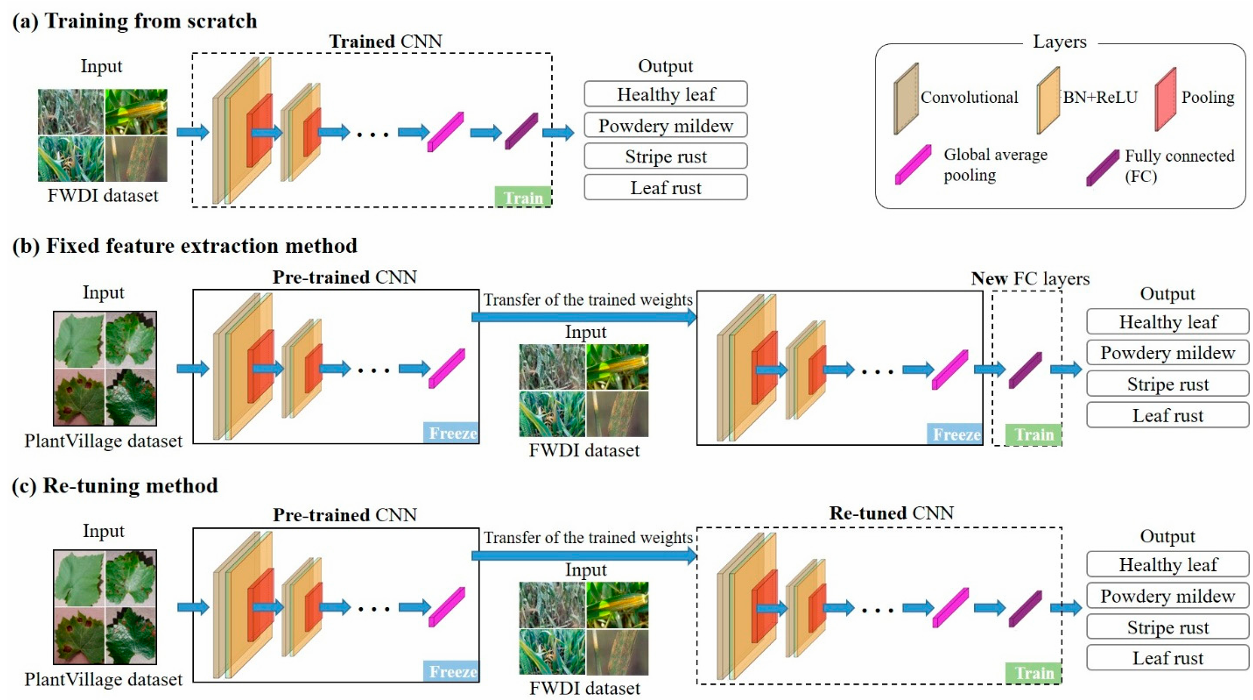
\includegraphics[width=1\textwidth]{chapters/chapter3/images/Figure03.png}
    \caption{Training strategies of a convolutional neural network (CNN) \parencite{jiang2022evaluation}.}
    \label{fig:TrainingStrategies}
\end{figure}



\textbf{Hybrid Models:} \parencite{nagpal2024hybrid} Introduced a hybrid model (Figure~\ref{fig:hybridframework}) that combines deep learning and traditional machine learning for image classification. Features are extracted from images using two pre-trained CNN models, MobileNet and DenseNet, and then concatenated. Particle Swarm Optimization (PSO) is applied for dimensionality reduction. Finally, the reduced features are fed into traditional classifiers (RF, SVM, DT) for training and prediction, achieving an accuracy of 98.89\% across four classes.


\begin{figure}[H] 
    \centering
    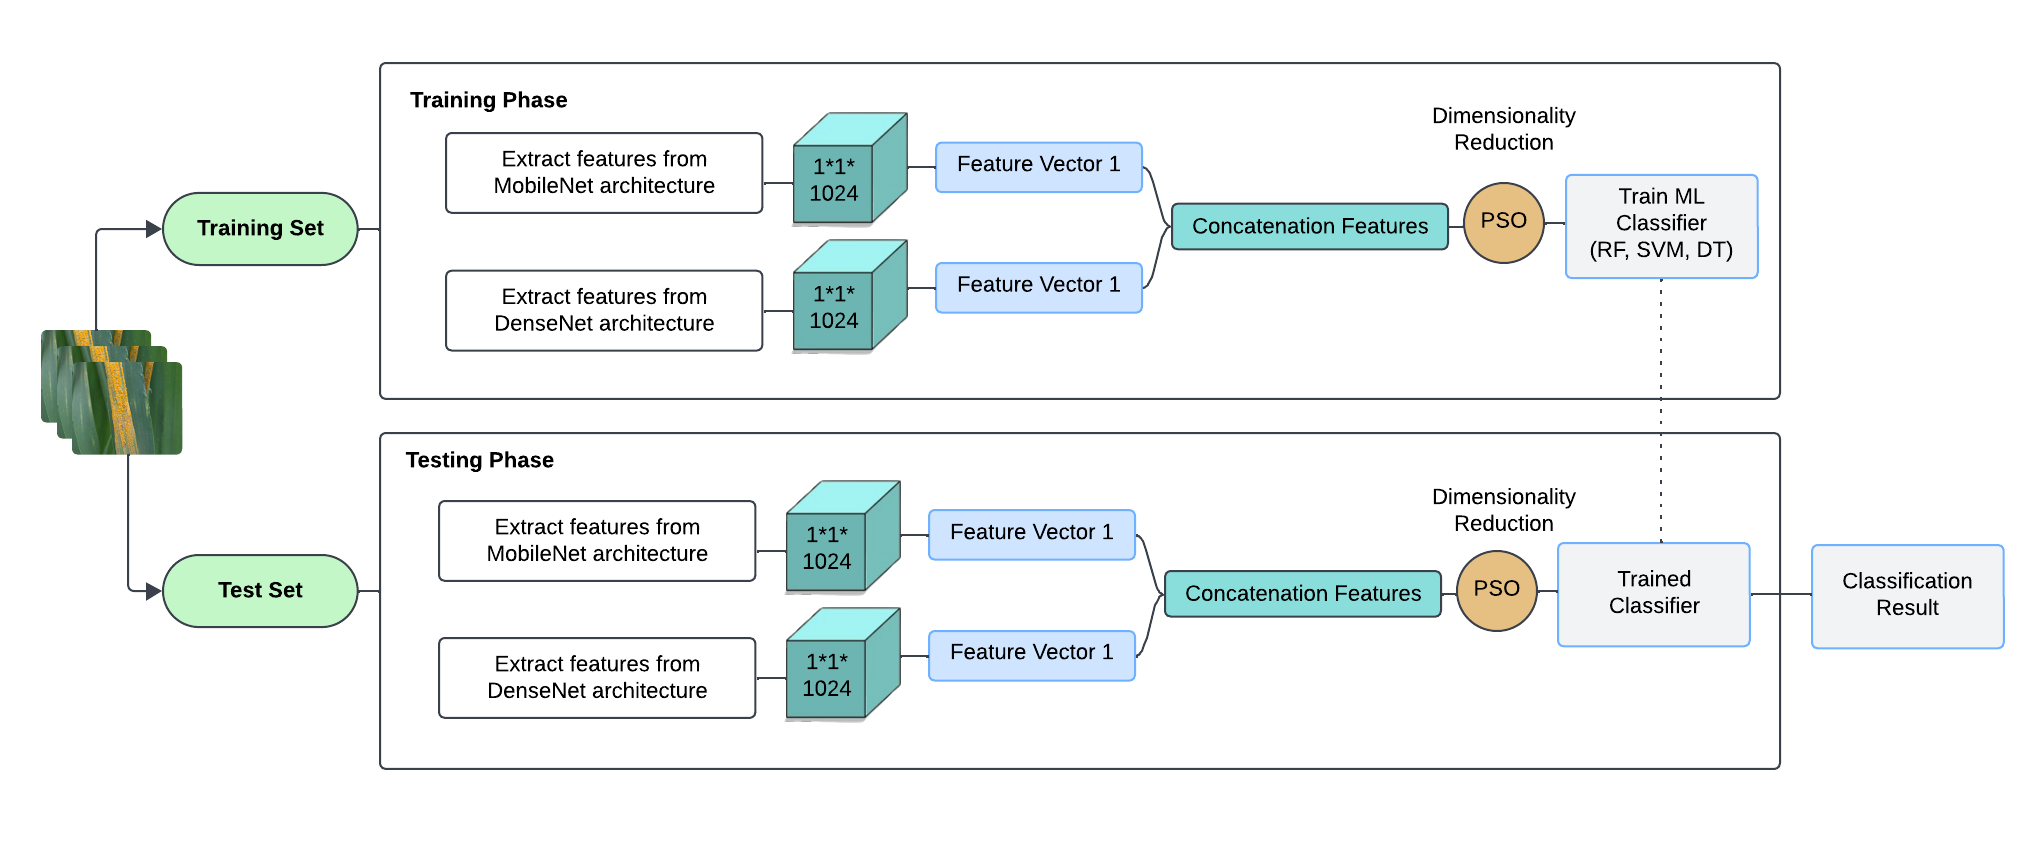
\includegraphics[width=1\textwidth]{chapters/chapter3/images/Figure04.png}
    \caption{The architecture of the hybrid framework \parencite{nagpal2024hybrid}.}
    \label{fig:hybridframework}
\end{figure}









\textbf{Custom Deep Convolutional Networks:} \parencite{goyal2021leaf} proposed a custom deep convolutional neural network (Figure~\ref{fig:CustomDeepCN}) specifically designed for wheat disease classification. The architecture comprises 21 convolutional layers, 7 max-pooling layers, and 3 fully connected layers. Activation functions used include ReLU and Leaky ReLU in the convolutional layers, while the fully connected layers employ ReLU, followed by a SoftMax classifier for multi-class output. The model was trained on a dataset of over 12,000 labeled RGB images covering 10 distinct wheat disease classes and achieved an accuracy of 97.88\%. 

\begin{figure}[H] 
    \centering
    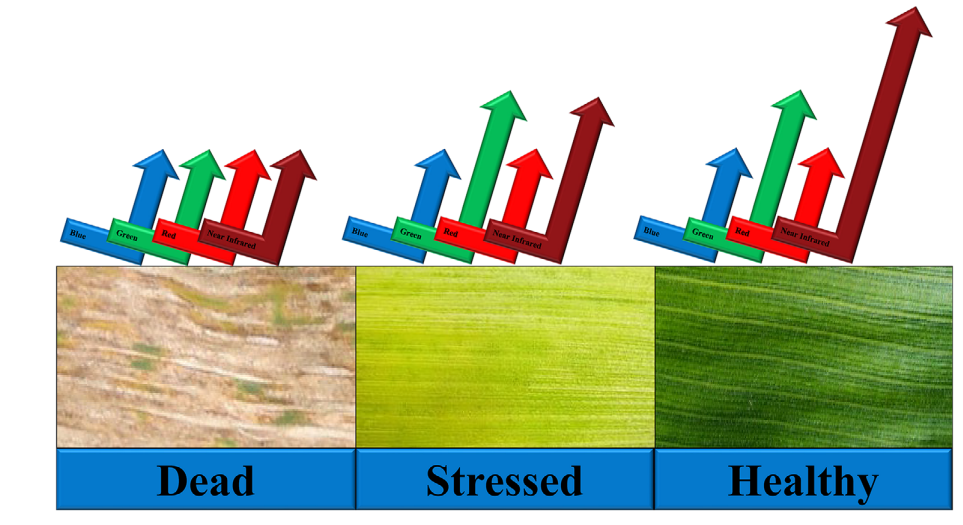
\includegraphics[width=0.8\textwidth]{chapters/chapter3/images/Figure05.png}
    \caption{The proposed deep convolutional neural network \parencite{goyal2021leaf}.}
    \label{fig:CustomDeepCN}
\end{figure}



\textbf{Few-Shot Learning:} \parencite{alharbi2023wheat} implemented a few-shot learning approach (Figure~\ref{fig:Few-shot}) using a Siamese network with EfficientNetB0 as a shared feature extractor to process both support and query images, generating feature embeddings for each. The support set contains a small number of labeled examples per class, while the query set includes unlabeled images to be classified. The Siamese structure ensures that the same feature extraction process is applied to both sets, enabling meaningful comparison. This model achieved an accuracy of 93.19\% in classifying 18 types of wheat diseases.


\begin{figure}[H] 
    \centering
    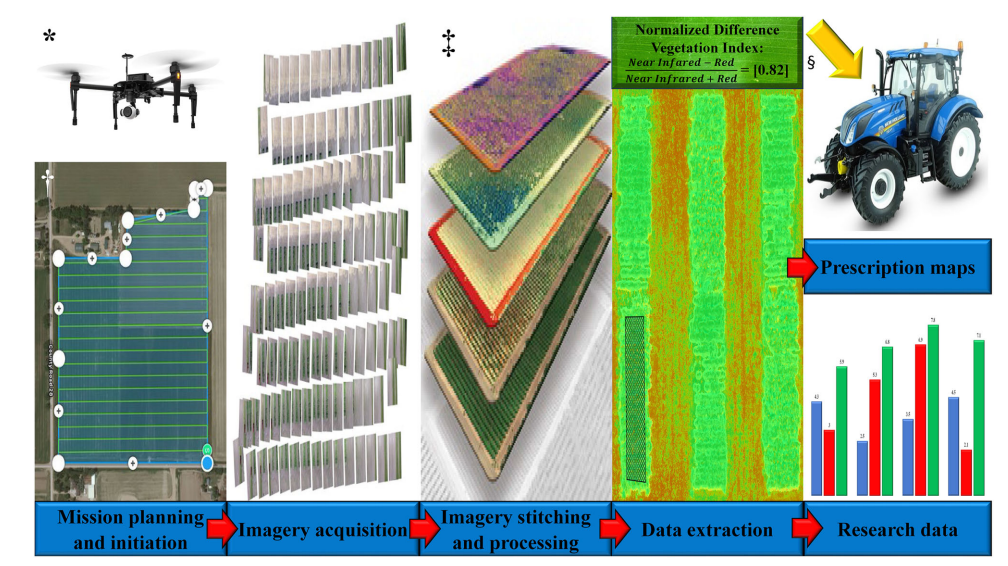
\includegraphics[width=0.9\textwidth]{chapters/chapter3/images/Figure06.png}
    \caption{Architecture diagram of a Few-shot Learning-based network \parencite{alharbi2023wheat}.}
    \label{fig:Few-shot}
\end{figure}


\textbf{Lightweight CNNs for Efficient Classification:} \parencite{fang2023lightweight} introduced a lightweight multiscale CNN model optimized for mobile and edge computing applications. By integrating Inception modules with residual blocks and attention mechanisms like Convolutional Block Attention Model (CBAM) and Efficient Channel Attention (ECA), the model enhanced feature extraction while reducing computational costs, achieving 98.78\% accuracy on wheat disease classification tasks​. Likewise, \parencite{jouini2023wheat} proposed a deep learning approach using MobileNetV2 and EfficientNet variants to build a lightweight yet accurate CNN-based model for wheat leaf disease detection in smart agriculture, achieving 94\% test accuracy.




\begin{table}[htbp]
    \caption{Related Work on Wheat Disease Classification}
    \centering
    \resizebox{\textwidth}{!}{%
    \begin{tabular}{|p{2cm}|p{6cm}|p{4.5cm}|p{1.5cm}|p{3.5cm}|p{2.5cm}|p{2cm}|}
    \hline
    \textbf{Reference} & \textbf{Approach} & \textbf{Image Preprocessing} & \textbf{Size (images)} & \textbf{Categories} & \textbf{Dataset} & \textbf{Results} \\
    \hline
    \parencite{ramadan2024improving} & Pre-trained CNNs (DenseNet121, ResNet50V2, MobileNetV2, Xception) & Data Augmentation (CycleGAN, ADASYN, SMOTE, SMOTETomek) & 407 & 3 (healthy, stripe rust, septoria) & Wheat Leaf Dataset & CycleGAN-augmented + MobileNetV2: 100\% accuracy \\
    \hline
    \parencite{nagpal2024hybrid} & Hybrid (MobileNet + DenseNet + PSO + SVM/DT/RF) & Resize 224x224, normalization, augmentation (cropping, flipping, rotation, noise, zooming) & 887 & 4 (yellow rust, brown rust, loose smut, healthy) & Custom Dataset & 98.89\% \\
    \hline
    \parencite{reis2024integrated} & Deep models + Ensemble learning & CLAHE, hypercolumn & 2400 & 3 (healthy, yellow rust, brown rust) & Wheat Disease Detection Dataset & 99.72\% \\
    \hline
    \parencite{goyal2021leaf} & Improved deep CNN architecture & / & 12,000 & 10 (e.g., karnal bunt, powdery mildew, healthy...) & LWDCD2020 & 97.88\% \\
    \hline
    \parencite{alharbi2023wheat} & Few-shot learning with EfficientNet and attention & / & 1530 & 18 classes & PlantVillage, CGIAR, manual, Google Images & 93.19\% \\
    \hline
    \parencite{jouini2024wheat} & CropNet (EfficientNetB0 + shallow CNN layers) & Resize 256x256, StandardScaler normalization & / & 5 (healthy, septoria, mildew, brown/yellow rust) & / & 99.80\% \\
    \hline
    \parencite{fang2023lightweight} & Inception-ResNet-CE with CBAM/ECA attention & Contrast enhancement, data augmentation & $>$12,000 & 7 (healthy, rusts, powdery, smut...) & LWDCD2020, PlantVillage, CGIAR, Wheat Leaf & 98.76\% \\
    \hline
    \parencite{nigam2023deep} & EfficientNet transfer learning & Contrast enhancement, resize, augmentation & 6556 & 4 (stripe rust, stem rust, leaf rust, healthy) & WheatRust21 & 99.35\% \\
    \hline
    \parencite{jiang2022evaluation} & 7 CNNs evaluated (e.g., VGG-16, ResNet-50) & Resize 224x224, normalization, geometric augmentation & 2643 & 4 (healthy, mildew, rusts) & FWDI, PlantVillage & 92.5\% \\
    \hline
    \end{tabular}%
    }
    \label{tab:wheat-disease-related-work}
\end{table}
    


The studies are complementary as they address different challenges in wheat disease classification. Figure ~\ref{fig:Figure01} summarizes the main approaches used in this field, providing a taxonomy that includes transfer learning, hybrid models, custom CNN architectures, few-shot learning, lightweight CNNs, and attention mechanisms. Transfer learning helps overcome limited data by leveraging pre-trained models, while hybrid models combine deep learning and traditional machine learning to enhance performance. Custom and task-specific CNNs are tailored to the unique features of wheat diseases, improving accuracy. Few-shot learning enables effective classification with minimal labeled data, and lightweight CNNs optimize real-time detection for mobile and edge devices, balancing performance with computational efficiency. Each approach targets a specific problem, enhancing the overall classification process.    

\begin{figure}[H]
    \centering
    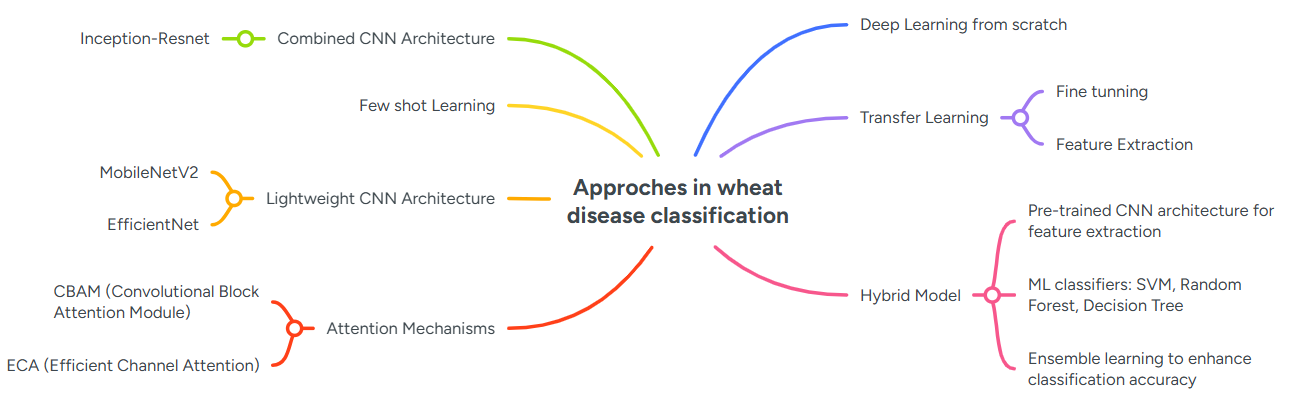
\includegraphics[width=1.0\textwidth]{chapters/chapter3/images/Figure09.png}
    \caption{Taxonomy of Approaches for Classifying Wheat Diseases. \protect\parencite{haider2021wheat}}
    \label{fig:Figure01}
\end{figure}


\section{Core Limitations and Research Gaps in Wheat Disease and Pest Detection}
Deep learning has shown great promise in automating wheat disease detection, offering timely and precise solutions for sustainable agriculture. However, key challenges still limit its widespread adoption.

Based on the previously discussed studies, various approaches have been explored for wheat disease classification, ranging from transfer learning using pre-trained convolutional neural networks (CNNs) to the development of custom architectures tailored specifically for disease classification tasks. The proposed models for wheat disease classification that detect five or fewer disease classes generally achieve accuracies of 99% or higher. However, models aiming to detect more than five classes tend to achieve lower accuracies, typically below 98%, highlighting the challenge of achieving high accuracy when dealing with more complex classification tasks.

Additionally, the number of disease classes addressed in most proposed models for wheat detection remains limited compared to the actual variety of diseases observed in the field, with a maximum of five classes, primarily due to the difficulty of manual annotation and the high computational resources required to train models on larger, more diverse datasets. Although several public datasets for wheat disease classification are available, such as those on Kaggle, these sources often contain low-quality images, inconsistent labeling, or irrelevant data, which can hinder model training and performance. This necessitates manual cleaning and preprocessing of the datasets before they can be effectively utilized, increasing the time and effort needed for research.

Moreover, the performance of these models is often affected by inconsistencies in image data. Therefore, diversifying image data is crucial; photos should be taken under varying lighting conditions, such as on sunny and cloudy days, and from different distances, including both close-up and wider shots. Creating a custom dataset by selecting diverse images from different public datasets is important to ensure this variability and improve model robustness.

Beyond dataset issues, several structural and architectural limitations remain. Most current models use a single-stage classification pipeline that attempts to identify all classes in one pass. This approach can be inefficient, especially when simple distinctions (e.g., healthy vs. diseased) could be resolved earlier using lightweight inference mechanisms. The lack of hierarchical or multi-stage classification pipelines presents an opportunity for improvement in computational efficiency and deployment readiness.

Furthermore, few models explicitly address deployment constraints such as low computational power, memory limitations, or real-time processing requirements, which are crucial for applications in edge computing or mobile agricultural tools used directly in the field. The absence of design considerations for lightweight architectures and early-exit strategies limits the practical applicability of many existing solutions.

Another significant limitation is the lack of evaluation on real-world field images that exhibit high variability in terms of background, illumination, occlusion, and resolution. While many models achieve excellent performance on curated datasets, their generalization to uncontrolled field conditions remains underexplored. Robustness under such conditions is essential for real-life adoption by farmers and agronomists.

Finally, although attention mechanisms and hybrid models have been proposed in recent literature, few studies explicitly quantify the trade-offs between accuracy and computational cost in multi-class settings, especially when scaling up to cover a wider range of diseases.

\section{Conclusion}
In conclusion, integrating image-based detection systems powered by advanced deep learning models presents a promising solution for combating wheat diseases and insect pests. The reviewed methodologies highlight the importance of data acquisition, preprocessing techniques, and model selection for accurate and efficient detection. While significant progress has been made, challenges such as dataset limitations, computational cost, and model generalization remain. Future research should improve model robustness, data augmentation strategies, and real-time deployment to facilitate practical applications in agricultural fields. As technology continues to evolve, these detection systems are expected to play an increasingly vital role in sustainable agriculture. 


% === Deuxième Partie: Contribution ===
\part{Contribution}
\include{chapters/chapter4/chapter4} % Conception
\include{chapters/chapter5/chapter5} % Réalisation


% Conclusion Générale
\chapter*{General conclusion}
\addcontentsline{toc}{chapter}{General conclusion}
\label{chap.general-conclusion}

The increasing global demand for wheat, coupled with the persistent threat of plant diseases and insect pests, underscores the urgent need for innovative and efficient monitoring systems in agriculture. Traditional disease detection methods, while useful, are often limited in scale, accuracy, and timeliness. This has prompted the adoption of smart agriculture technologies, particularly the integration of remote sensing with machine learning (ML) and deep learning (DL) techniques.

Throughout this report, we have examined how the fusion of aerial imagery—acquired through satellites, UAVs, and multispectral sensors—with advanced AI models enables early detection, classification, and monitoring of various wheat diseases. We have explored the fundamentals of DL and ML, including their roles in core computer vision tasks, and reviewed different imaging technologies used in precision agriculture.

Moreover, we discussed the challenges inherent in this integration, such as data heterogeneity, high computational demands, and the need for large annotated datasets. Despite these limitations, the results from existing studies demonstrate that remote sensing combined with AI holds immense potential for automated, scalable, and real-time disease detection systems.

In conclusion, the integration of remote sensing and intelligent algorithms is not only transforming the way we monitor crop health but also paving the way for sustainable, data-driven agricultural practices. Future work should focus on improving data fusion strategies, model generalization, and deploying lightweight solutions for field-level implementation—bringing us closer to the vision of fully autonomous smart farming systems.

% Bibliography
\printbibliography[heading=bibintoc]



% Appendices
\begin{appendices}
    \chapter{Dependencies and libraries}%
\label{app:annexA}

\begin{center}
    \begin{verbatim}
   annex a 
    \end{verbatim}
\end{center}
    \include{appendices/annexeB}
\end{appendices}

\end{document}